\chapter{Propuesta}\label{chapter:proposal}

El principal objetivo de este trabajo es la construcción de wavelets adaptadas a patrones usando el algoritmo de
la DST-II \cite{Guido2018} para su posterior detección en señales. En este capítulo se presenta una explicación 
detallada del algoritmo, así como varias propuestas para su extensión para el uso en señales bidimensionales para
ser luego aplicada específicamente para la detección de masas en mamografías.

\section{Aspectos generales de las DSTs}

La DST-II es una modificación de la DST. Por este motivo ambas comparten muchos puntos y de forma similar 
a la DWT poseen los siguientes componentes y características \cite{Guido2008}\cite{Guido2018}:

\begin{itemize}
	\item El par de filtros $p[\cdot]$ y $q[\cdot]$ donde $q_k = (-1)^k p_{N-k-1}$. 
		Estos representan ,respectivamente, los filtros \textit{low-pass} y \textit{high-pass} y  
		usados en conjunto con el algoritmo de Mallat \cite{} para obtener la transformada de la 
		señal, exactamente igual a como se hace en la DWT, donde se les conoce usualmente como $h[\cdot]$ y
		$g[\cdot]$.
	\item El par de filtros $\bar p[\cdot]$  y $\bar q[\cdot]$ que son los filtros usados para la etapa 
		de síntesis de la señal. En el ámbito de la DWT, se conocen como $\bar h[\cdot]$ y $\bar g[\cdot]$.
	\item Las funciones $\Gamma(x)=\sum_k p_k \Gamma(2N-k)$ y $\Theta(x)=\sum_k q_k \Theta(2N-k)$ conocidas 
		como \textit{major shapelet} y \textit{minor shapelet} respectivamente. Las mismas conrresponden a las
		funciones de \textit{scaling} $\phi(x)$ y \textit{wavelet} $\psi(x)$ en la DWT.
	\item Las condiciones $\bar P[z] = Q[-z]$, $\bar Q[z]=-P[-z]$ y $\bar P[z]P[z] + \bar Q[z]Q[z]=2z^{-N+1}$,
		todas en el dominio de $Z$, implican que $p[\cdot]$, $q[\cdot]$, $\bar p[\cdot]$  y $\bar q[\cdot]$
		forman un banco de filtro de construcción perfecta (PRFB por sus siglas en inglés).
\end{itemize}

Otro aspecto importante de las DST es que el resultado de la misma al procesar una señal $s[\cdot]$ produce dos 
señales de igual longitud igual a la mitad de la señal de entrada $s[\cdot]$. La primera mitad corresponde a 
\textit{master} y la segunda a \textit{second-rated}. La concatenación de las mismas caracteriza a las DST
y corresponden a los coeficientes de aproximación y detalles en la DWT respectivamente.

El procedimiento para obtener el filtro $q[\cdot]$ de la DST-II es similar al usado para generar el mismo filtro
en la DST. Sin embargo, la condición basada en el \textit{matching} fractal es sustuida por un par de condiciones
conocidas como \textit{matching conditions}.


\section{Formulación de la DST-II}\label{algoritmo:dst-2}

Como se menciona en la sección anterior, el procedimiento para obtener el filtro $q[\cdot]$ en la DST y DST-II
es distinto. Para el cálculo del mismo se establecen las siguientes restricciones:

\begin{itemize}
	\item El tamaño del filtro debe ser ser $N \geq 6$. Esta restricción es necesaria por el hecho de que la 
		DST-II tiene $\frac{N}{2}-2$  momentos nulos su \textit{minor shapelet}, equivalente a función \textit{wavelet}
		en la DWT. Por tanto, si $N<6$, no se tendrían momentos nulos en esa función, distorsionando la transformada.
	\item El tamaño del filtro deber ser par, al igual que en la DWT. De lo contrario, no se puede obtener una 
		reconstrucción perfecta.
	\item El patrón que se quiere detectar $m[\cdot]$, debe tener tamaño impar igual a $N+1$.
\end{itemize}

Teniendo en cuenta las restricciones anteriores, el procedimiento para la obtención del filtro $q[\cdot]$ en la DST-II 
es el siguiente:

\begin{itemize}
	\item \textbf{Paso 1:} Forzar que el filtro posea energía unitaria
		\begin{equation}\label{eq:unitary-energy}
			\sum_{k=0}^{N-1}q_k^2 = 1.
		\end{equation}
	\item \textbf{Paso 2:} Imponer $\frac{N}{2} -2 $ momentos nulos para la \textit{mejor shapelet}
		\begin{equation}\label{eq:vanishing-moments}
			\sum_{k=0}^{N-1}q_{k}k^b = 0
		\end{equation}
		donde $b=0,1,\dotsc,\frac{N}{2}-3$.
	\item \textbf{Paso 3:} Definir las condiciones de otogonalidad
		\begin{equation}\label{eq:orthogonality}
			\sum_{0}^{N-1} q_{k}q_{k+2l} = \delta_{0,1}
		\end{equation}
		donde $\delta$ es el delta de Dirac y $l\in Z$.
	\item \textbf{Paso 4:} Agregar las condiciones de \textit{matching}
		\begin{equation}\label{eq:matching-1}
			\sum_{0}^{N-1} q_{k}m_{k} = 0
		\end{equation}
		\begin{equation}\label{eq:matching-2}
			\sum_{0}^{N-1} q_{k}m_{k+1} = 0
		\end{equation}
	\item \textbf{Paso 5:} Agrupar todas las ecuaciones definidas anteriormente y resolver el sistema de ecuaciones
		no lineales $N$ ecuaciones y $N$ incógnitas para obtener el filtro $q[\cdot]$.
	\item \textbf{Paso 6:} Obtener $p[\cdot]$ como $p_k=(-1)^{k+1}q_{N-k-1}$ y 
		después a partir de $q[\cdot]$ y $p[\cdot]$ calcular los filtros $\bar q[\cdot]$ y $\bar p[\cdot]$.
	\item \textbf{Paso 7:} Como paso opcional, si se desea conocer la forma de la \textit{major} y \textit{minor}
		\textit{shapelet} se pueden calcular $\Gamma(x)=\sum_k p_k \Gamma(2N-k)$ y $\Theta(x)=\sum_k q_k \Theta(2N-k)$.
\end{itemize}

En esencia la DST-II corresponde a la transformada de Daubechies, cambiando de de los momentos nulos por las
condiciones de \textit{matching},\ref{eq:matching-1} y \ref{eq:matching-2}. Estas están definidas de forma tal que el
producto inherente como resultado del cómputo de la DST-II, basado en el algoritmo de Mallat, reaccione ante 
la presencia del patrón $m[\cdot]$.

El algoritmo de la DST-II y su inversa es exactamente el mismo que para la DWT, por lo que la complejidad computacional
es la misma.

\section{Solución numérica del sistema de ecuaciones no lineales}\label{numerical-solution}

Solucionar un sistema de ecuaciones no lineales, es una situación que se evita siempre que sea posible. Por lo general
se trata de simplificar el sistema sustituyendolo con uno lineal \cite{Burden2016}. Sin embargo, esto no siempre es posible y se debe abordar el problema de
forma directa. En el caso de la construcción del filtro $q$, no es posible simplificar el sistema, pues violaría
las condiciones de su propia definición. Por este motivo es necesario seleccionar métodos numéricos para la
solución del sistema definido en \ref{algoritmo:dst-2}.

El método de Newton es de los más simples y conocidos para resolver ecuaciones y se puede extender al caso de varias
variables. Su convergencia suele ser rápida una vez que se obtiene una aproximación que está cerca de la solución
verdadera. Sin embargo, no siempre es fácil determinar un conjunto de valores iniciales. Además, otra debilidad
significativa para resolver sistemas de ecuaciones no lineales es la necesidad de determinar en cada iteración 
una matriz y resolver un sistema lineal de tamaño $n\times n$ \cite{Burden2016}. 

Existe otra clase de algoritmos llamados métodos de Newton inexactos o cuasi-Newton. Estos métodos reemplazan la
matriz jacobian en el método de Newton con una matriz de aproximación que se actualiza fácilmente en 
cada iteración. La desventaja de estos métodos es que la convergencia cuadrática del método de Newton se pierde,
al ser reemplazada, en general, mediante una convergencia superlineal. Otra desventaja es que a diferencia 
del método de Newton, los métodos quasi-Newton no se autocorrigen. En muchos casos, el método de Newton
corrige el error de redondeo con iteraciones sucesivas. Sin embargo, en muchos escenarios, la reducción 
de la convergencia es un precio aceptable a pagar para reducir la cantidad de cálculos \cite{Burden2016}. 

Entre los métodos que pertenecen a esta clase de algoritmos se encuentran Broyden1 y Broyden2. El primero es conocido
como el método bueno de Broyden, y usa el primer jacobiano de Broyden para la aproximación. El segundo se conoce
como el método malo de Broyden, en vez del primer jacobiano, usa el segundo \cite{broyden}.

El método de Anderson también llamado Anderson \textit{mixing} \cite{Eyert1996} y el de Krylov también son métodos inexactos de Newton. 
Este último usa la aproximación de Krylov para el inverso del jacobiano y suele ser una buena opción para problemas
con de gran escala \cite{kelley1995iterative}.

Aunque el sistema planteado en \ref{algoritmo:dst-2} tiene exactamente la misma cantidad de ecuaciones que de 
incógnitas, algoritmos como el método híbrido de Powell y el algoritmo de Levenberg-Marquardt pueden 
ser usados para encontrar una solución. Ambos métodos están diseñados para problemas de mínimos cuadrados no lineales.

El algoritmo de Levenberg-Marquardt combina dos algoritmos de minimización numérica:
gradiente descendiente y el método de Gauss-Newton. El método Levenberg-Marquardt actúa más como gradiente 
descendiente cuando los parámetros están lejos del valor óptimo, y a medida que los valores se acercan 
al óptimo, actúa más como el método de Gauss-Newton \cite{madsen2004methods}.

El método híbrido de Powell, de forma similar a Levenberg-Marquardt es una combinación de gradiente descendiente y Gauss-Newton.
Sin embargo, en este la selección es controlada por el uso de una región de confianza \cite{madsen2004methods}.

\section{Heurística para la detección}

Al estar basada en la DWT, el análisis temporal y de frecuencia de la DST-II es exactamente igual que al de la DWT.
Sin embargo, la mayor novedad de este algoritmo, es la capacidad de reaccionar ante la presencia de 
patrones específicos, facilitando su detección. El proceso es bastante sencillo :
mientras más cercano a $0$ esté el coeficiente de la parte \textit{second-rated} de la transformada, más se parece
la sección de la señal analizada $s[\cdot]$ al patrón $m[\cdot]$ que se quiere detectar. En \cite{Guido2018} se
propone la siguiente función para la detección de las muestras que cumplan con estas características:

\begin{equation}
	\mathbb{S} = e^{-{(|DST-II(s[\cdot])|)}^{\alpha}} \ 0 < \alpha \leq 1
\end{equation}\label{eq:s-heuristic}

Mientras cercano sea $\mathbb{S}$ a 0 o 1, respectivamente, menos o más se parece el segmento de
la señal analizada $s[\cdot]$ a $m[\cdot]$.

Según \cite{Guido2018}, para el primer nivel de la DST-II, si $\mathbb{S}_{_k}=1$ para algún $k=0,1,2,\ldots$
con $k$ que pertenece a la segunda parte de la transformada ( \textit{second-rated} ), esto implica que 
que el patrón empieza en la posición $s_{2k-1}$ o $s_{2k}$. Un aspecto importante es que la búsqueda de 
ceros en la DST-II, o unos en $\mathbb{S}$, solo se lleva a cabo en la segunda sub-banda de la transformada,
es decir, en el segmento perteneciente a la \textit{second-rated}.

\section{Reajuste en las condiciones de \textit{matching}}

La DST-II está diseñada para que las condiciones de \textit{matching} \ref{eq:matching-1} \ref{eq:matching-2} 
permitan obtener un valor lo más cercano a $0$ cuando se realiza la convolución entre el filtro $q[\cdot]$
y el patrón $m[\cdot]$. Sin embargo, es necesario hacer un pequeño cambio a las ecuaciones \ref{eq:matching-1}
para que esto funcione \ref{eq:matching-1}.

De \ref{eq:mallat-details} se tiene que la convolución se hace multiplicando el filtro de atrás hacia adelante 
con la sección de la señal que se está procesando. Por lo que en vez usar las ecuaciones \ref{eq:matching-1}
y \ref{eq:matching-2} se usaron las siguientes:

\begin{equation}\label{eq:matching-1}
	\sum_{0}^{N-1} q_{-k}m_{k} = 0
\end{equation}
\begin{equation}\label{eq:matching-2}
	\sum_{0}^{N-1} q_{-k}m_{k+1} = 0
\end{equation}

\section{Ejemplo numérico del diseño de la DST-II}

\begin{figure} 
	\centering
	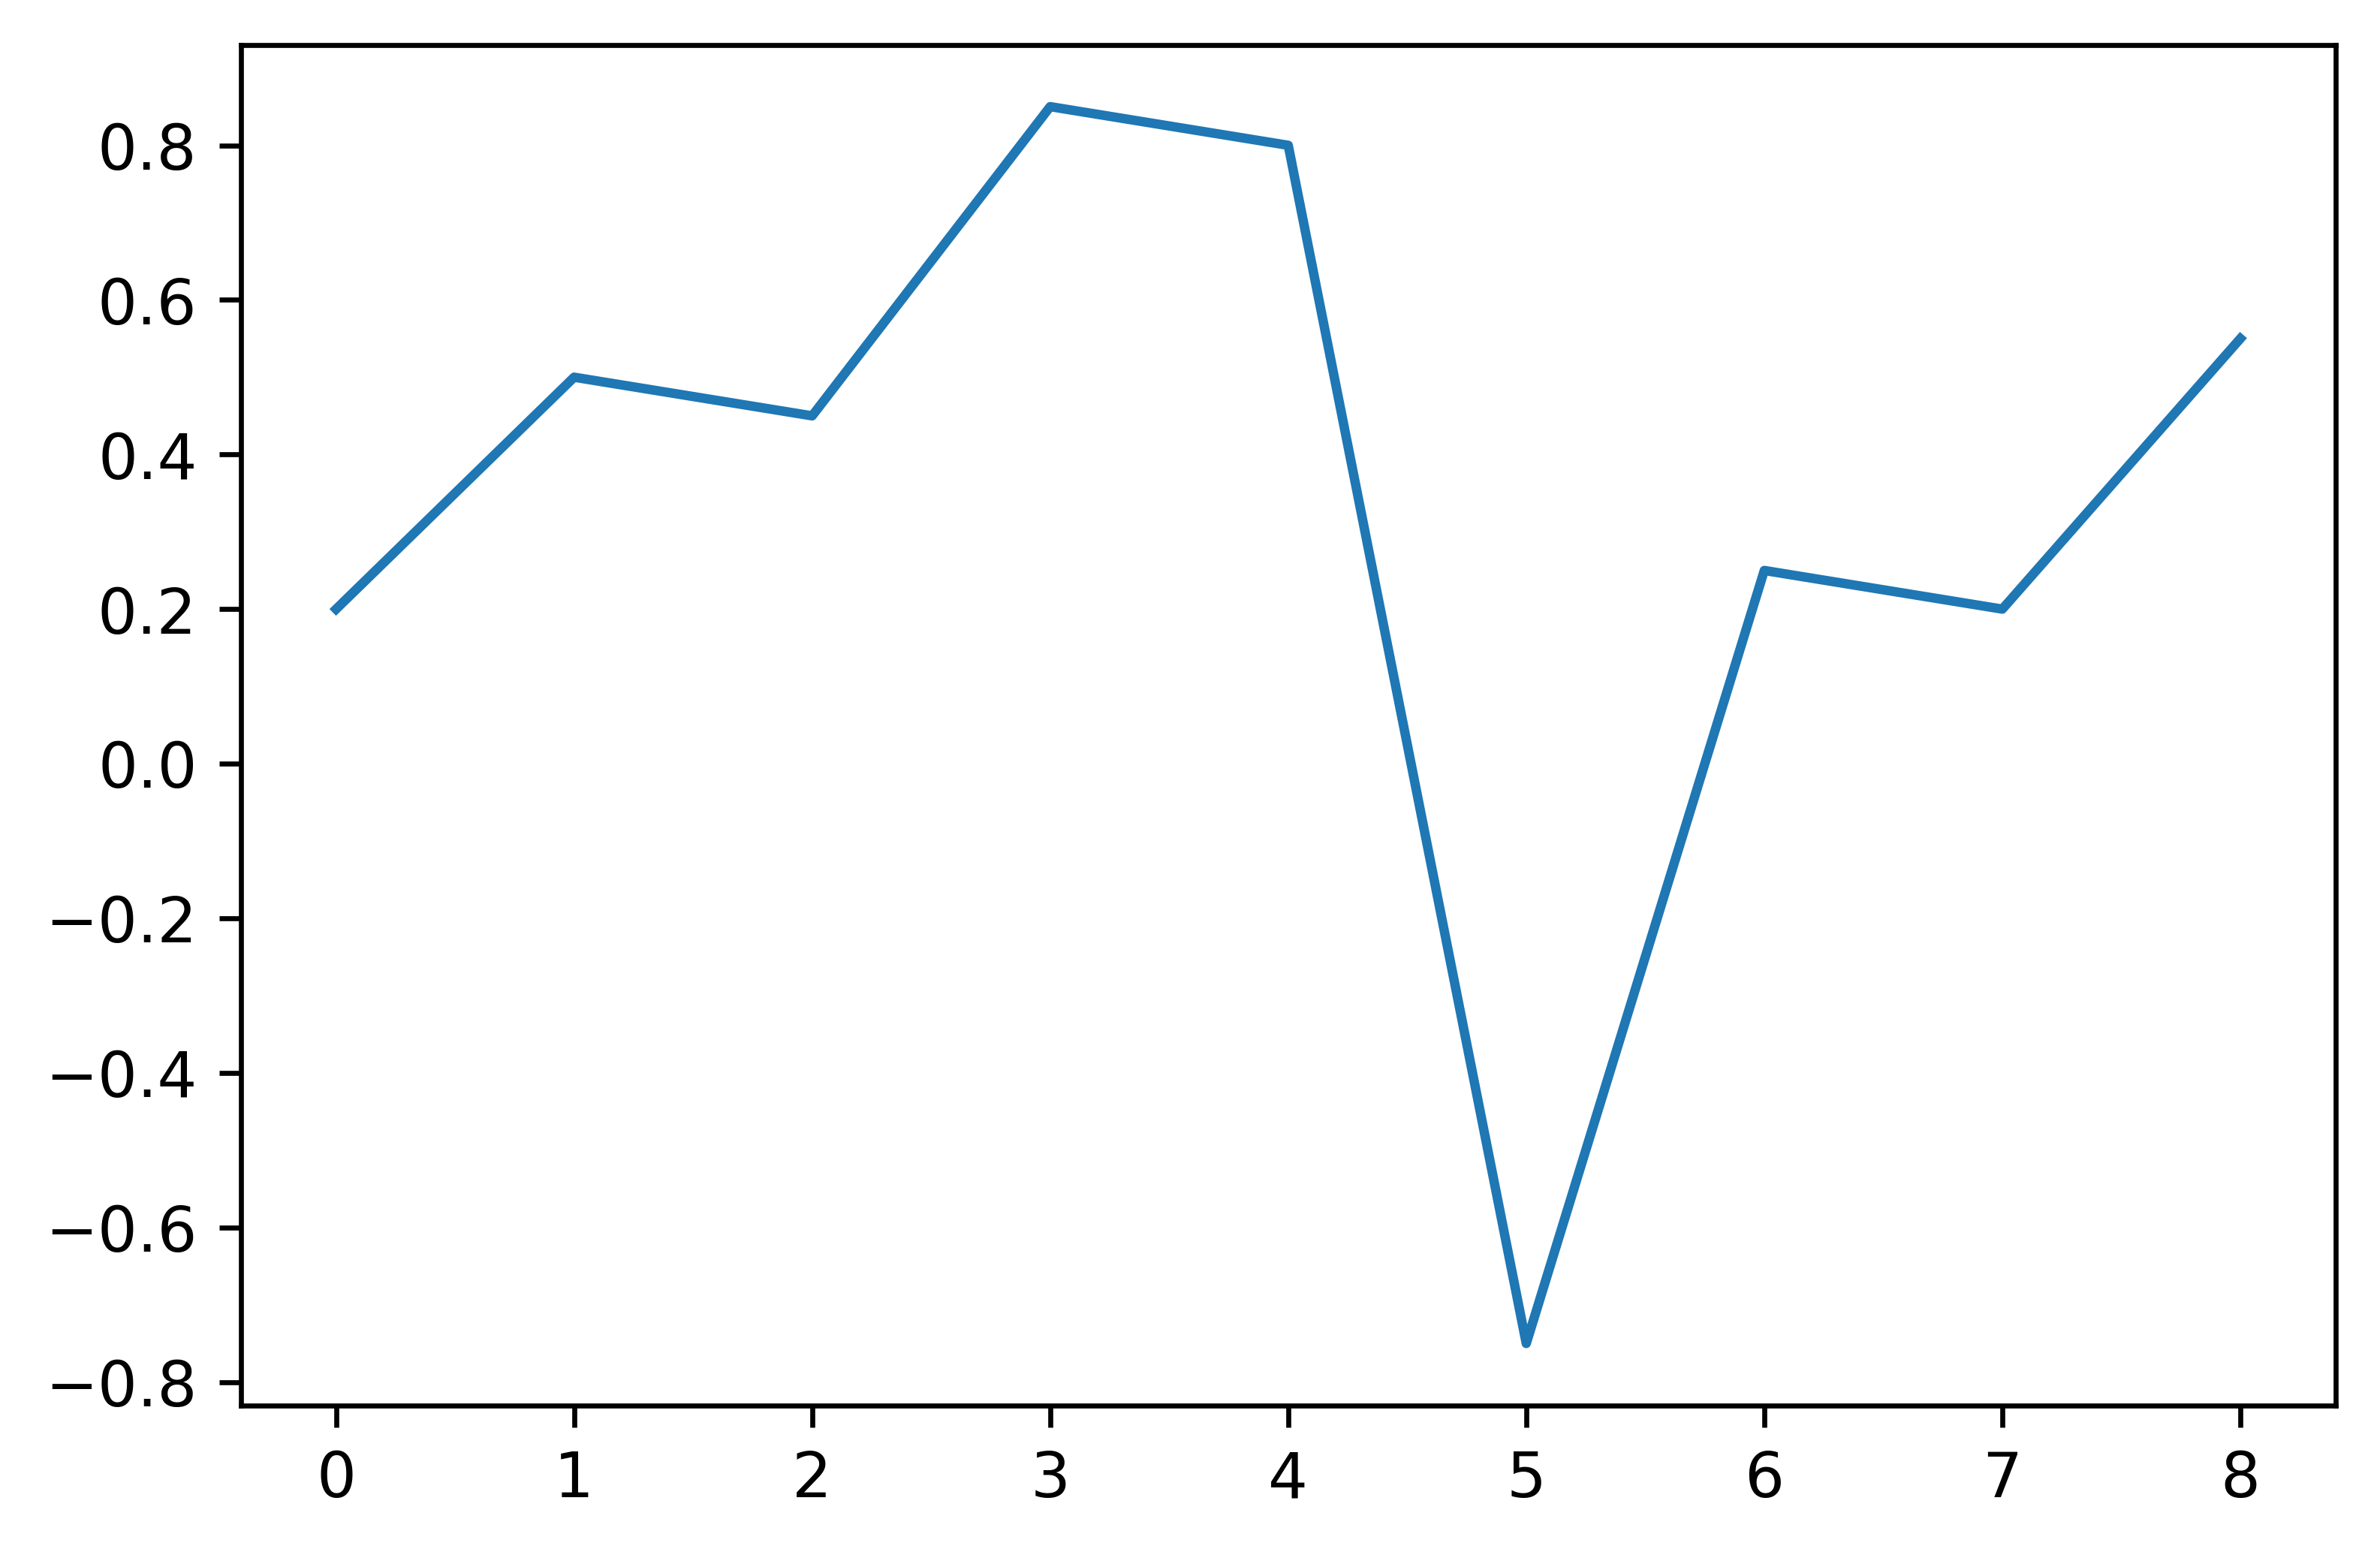
\includegraphics[scale=0.8]{Graphics/guido20118-pattern.png}
	\caption{Patrón usado en \cite{Guido2018} con valores [0.20, 0.50, 0.45, 0.85, 0.80, -0.75, 0.25, 0.20, 0.55]}\label{fig:Guido2018-pattern}
\end{figure}

En esta sección se describe paso a paso la construcción del filtro $q[\cdot]$ para la detección del
patrón $m[\cdot]$ que se muestra en \ref{fig:Guido2018-pattern}. 

Según los pasos descritos en \ref{algoritmo:dst-2}, las ecuaciones del sistema son las siguientes:

\begin{itemize}
	\item \textbf{Paso 1:} La ecuación de la energía unitaria \ref{eq:unitary-energy}
		\begin{equation}
			q_0^2 + q_1^2 + q_2^2 + q_3^2 + q_4^2 + q_5^2 + q_6^2 + q_7^2 - 1 = 0
		\end{equation}
	\item \textbf{Paso 2:} Dos ecuaciones de momentos nulos \ref{eq:vanishing-moments}
		\begin{equation}
			q_1 + q_2 + q_3 + q_4 + q_5 + q_6 + q_7  = 0
		\end{equation}
		\begin{equation}
			q_1 + 2q_2 + 3q_3 + 4q_4 + 5q_5 + 6q_6 + 7q_7 = 0
		\end{equation}
	\item \textbf{Paso 3:} Tres ecuaciones para las condiciones de ortogonalidad \ref{eq:orthogonality}
		\begin{equation}
			q_0q_2 + q_1q_3 + q_2q_4 + q_3q_5 + q_4q_6 + q_5q_7 = 0
		\end{equation}
		\begin{equation}
			q_0q_4 + q_1q_5 + q_2q_6 + q_3q_7 = 0
		\end{equation}
		\begin{equation}
			q_0q_6 + q_1q_7 = 0
		\end{equation}
	\item \textbf{Paso 4:} Las condiciones de \textit{matching} 
		\begin{equation}
			0.2q_0 + 0.2q_1 + 0.5q_2 + 0.45q_3 + 0.85q_4 + 0.8q_5 - 0.75q_6 + 0.25q_7 = 0
		\end{equation}
		\begin{equation}
			0.55q_0 + 0.5q_1 + 0.45q_2 + 0.85q_3 + 0.8q_4 - 0.75q_5 + 0.25q_6 + 0.2q_7 = 0
		\end{equation}
	\item \textbf{Paso 5:} Agrupando todas las ecuaciones se obtiene el sistema de ecuaciones no lineales
		\begin{equation}\label{eq:system}
			\left\{ \begin{array}{rcl}
						q_0^2 + q_1^2 + q_2^2 + q_3^2 + q_4^2 + q_5^2 + q_6^2 + q_7^2 - 1 = 0 \\
						q_1 + q_2 + q_3 + q_4 + q_5 + q_6 + q_7  = 0 \\
						q_1 + 2q_2 + 3q_3 + 4q_4 + 5q_5 + 6q_6 + 7q_7 = 0 \\
						q_0q_2 + q_1q_3 + q_2q_4 + q_3q_5 + q_4q_6 + q_5q_7 = 0 \\
						q_0q_4 + q_1q_5 + q_2q_6 + q_3q_7 = 0 \\
						q_0q_6 + q_1q_7 = 0 \\
						0.2q_0 + 0.2q_1 + 0.5q_2 + 0.45q_3 + 0.85q_4 + 0.8q_5 - 0.75q_6 + 0.25q_7 = 0 \\
						0.55q_0 + 0.5q_1 + 0.45q_2 + 0.85q_3 + 0.8q_4 - 0.75q_5 + 0.25q_6 + 0.2q_7 = 0 \\
					\end{array}
				\right.
			\end{equation}
\end{itemize}

Luego de resolver el \ref{eq:system} se obtiene como solución el siguiente vector para $q[\cdot]$:

$$
	\begin{array}{lcl}
		q[\cdot] = \{ 0.02135806, 0.23273233,  0.08239873, -0.80643852,  0.5152966,  -0.11358755, \\
		0.09865178, -0.00905336 \}
	\end{array}
$$

Una vez que se tiene el valor de $q[\cdot]$ se procede a calcular el resto de los filtros:

$$
	\begin{array}{lcl}
		p[\cdot] = \{ 0.00905336326604119, 0.09865177980292716, 0.11358755363902126,\\
			0.5152966037304808, 0.8064385205411737, 0.08239872502860128, \\
		-0.23273232888422687, 0.021358056806980778 \}
	\end{array}
$$

$$
	\begin{array}{lcl}
		\bar p[\cdot] = \{ 0.00905336326604119, 0.021358056806980778, -0.23273232888422687, \\
			0.08239872502860128, 0.8064385205411737, 0.5152966037304808,  \\ 
		0.11358755363902126, 0.09865177980292716 \}
	\end{array}
$$

$$
	\begin{array}{lcl}
		\bar q[\cdot] = \{ 0.021358056806980778, -0.00905336326604119, 0.09865177980292716, \\
			-0.11358755363902126, 0.5152966037304808, -0.8064385205411737, \\
		0.08239872502860128, 0.23273232888422687 \}
	\end{array}
$$

Un vez se obtienen los filtros, es posible realizar la DST-II sobre cualquier señal para detectar la presencia
del patrón $m[\cdot]$. Como paso opcional si se quiere obtener las funciones \textit{major} y \textit{minor}
se procedería a resolver los sistemas formados por las eucaciones  $\Gamma(x)=\sum_k p_k \Gamma(2N-k)$ y 
$\Theta(x)=\sum_k q_k \Theta(2N-k)$.

\section{Ejemplo de la aplicación de la DST-II}

Para demostrar el uso de las DST-II en la detección de patrones y formas, el patrón $m[\cdot]$ \ref{fig:Guido2018-pattern} fue
insertado en la señal $s[\cdot]$, dando como resultado la siguiente señal \ref{fig:example-guido-signal}:

\begin{equation}
	s[x] = \left\{ \begin{array}{rcl}
			\cos{\frac{27\pi x}{8}}\sin{\frac{75\pi x}{8}} & \mbox{si} &  0\leq x \leq 40 \\
			m[x]    &    \mbox{si}     &     41\leq x \leq 49     \\
			\cos{\frac{295\pi x}{32}}\sin{\frac{105\pi x}{32}} & \mbox{si} &  50\leq x \leq 63 \\
					 \end{array}
	\right.
\end{equation}


\begin{figure}\label{fig:example-guido-signal}
	\centering
	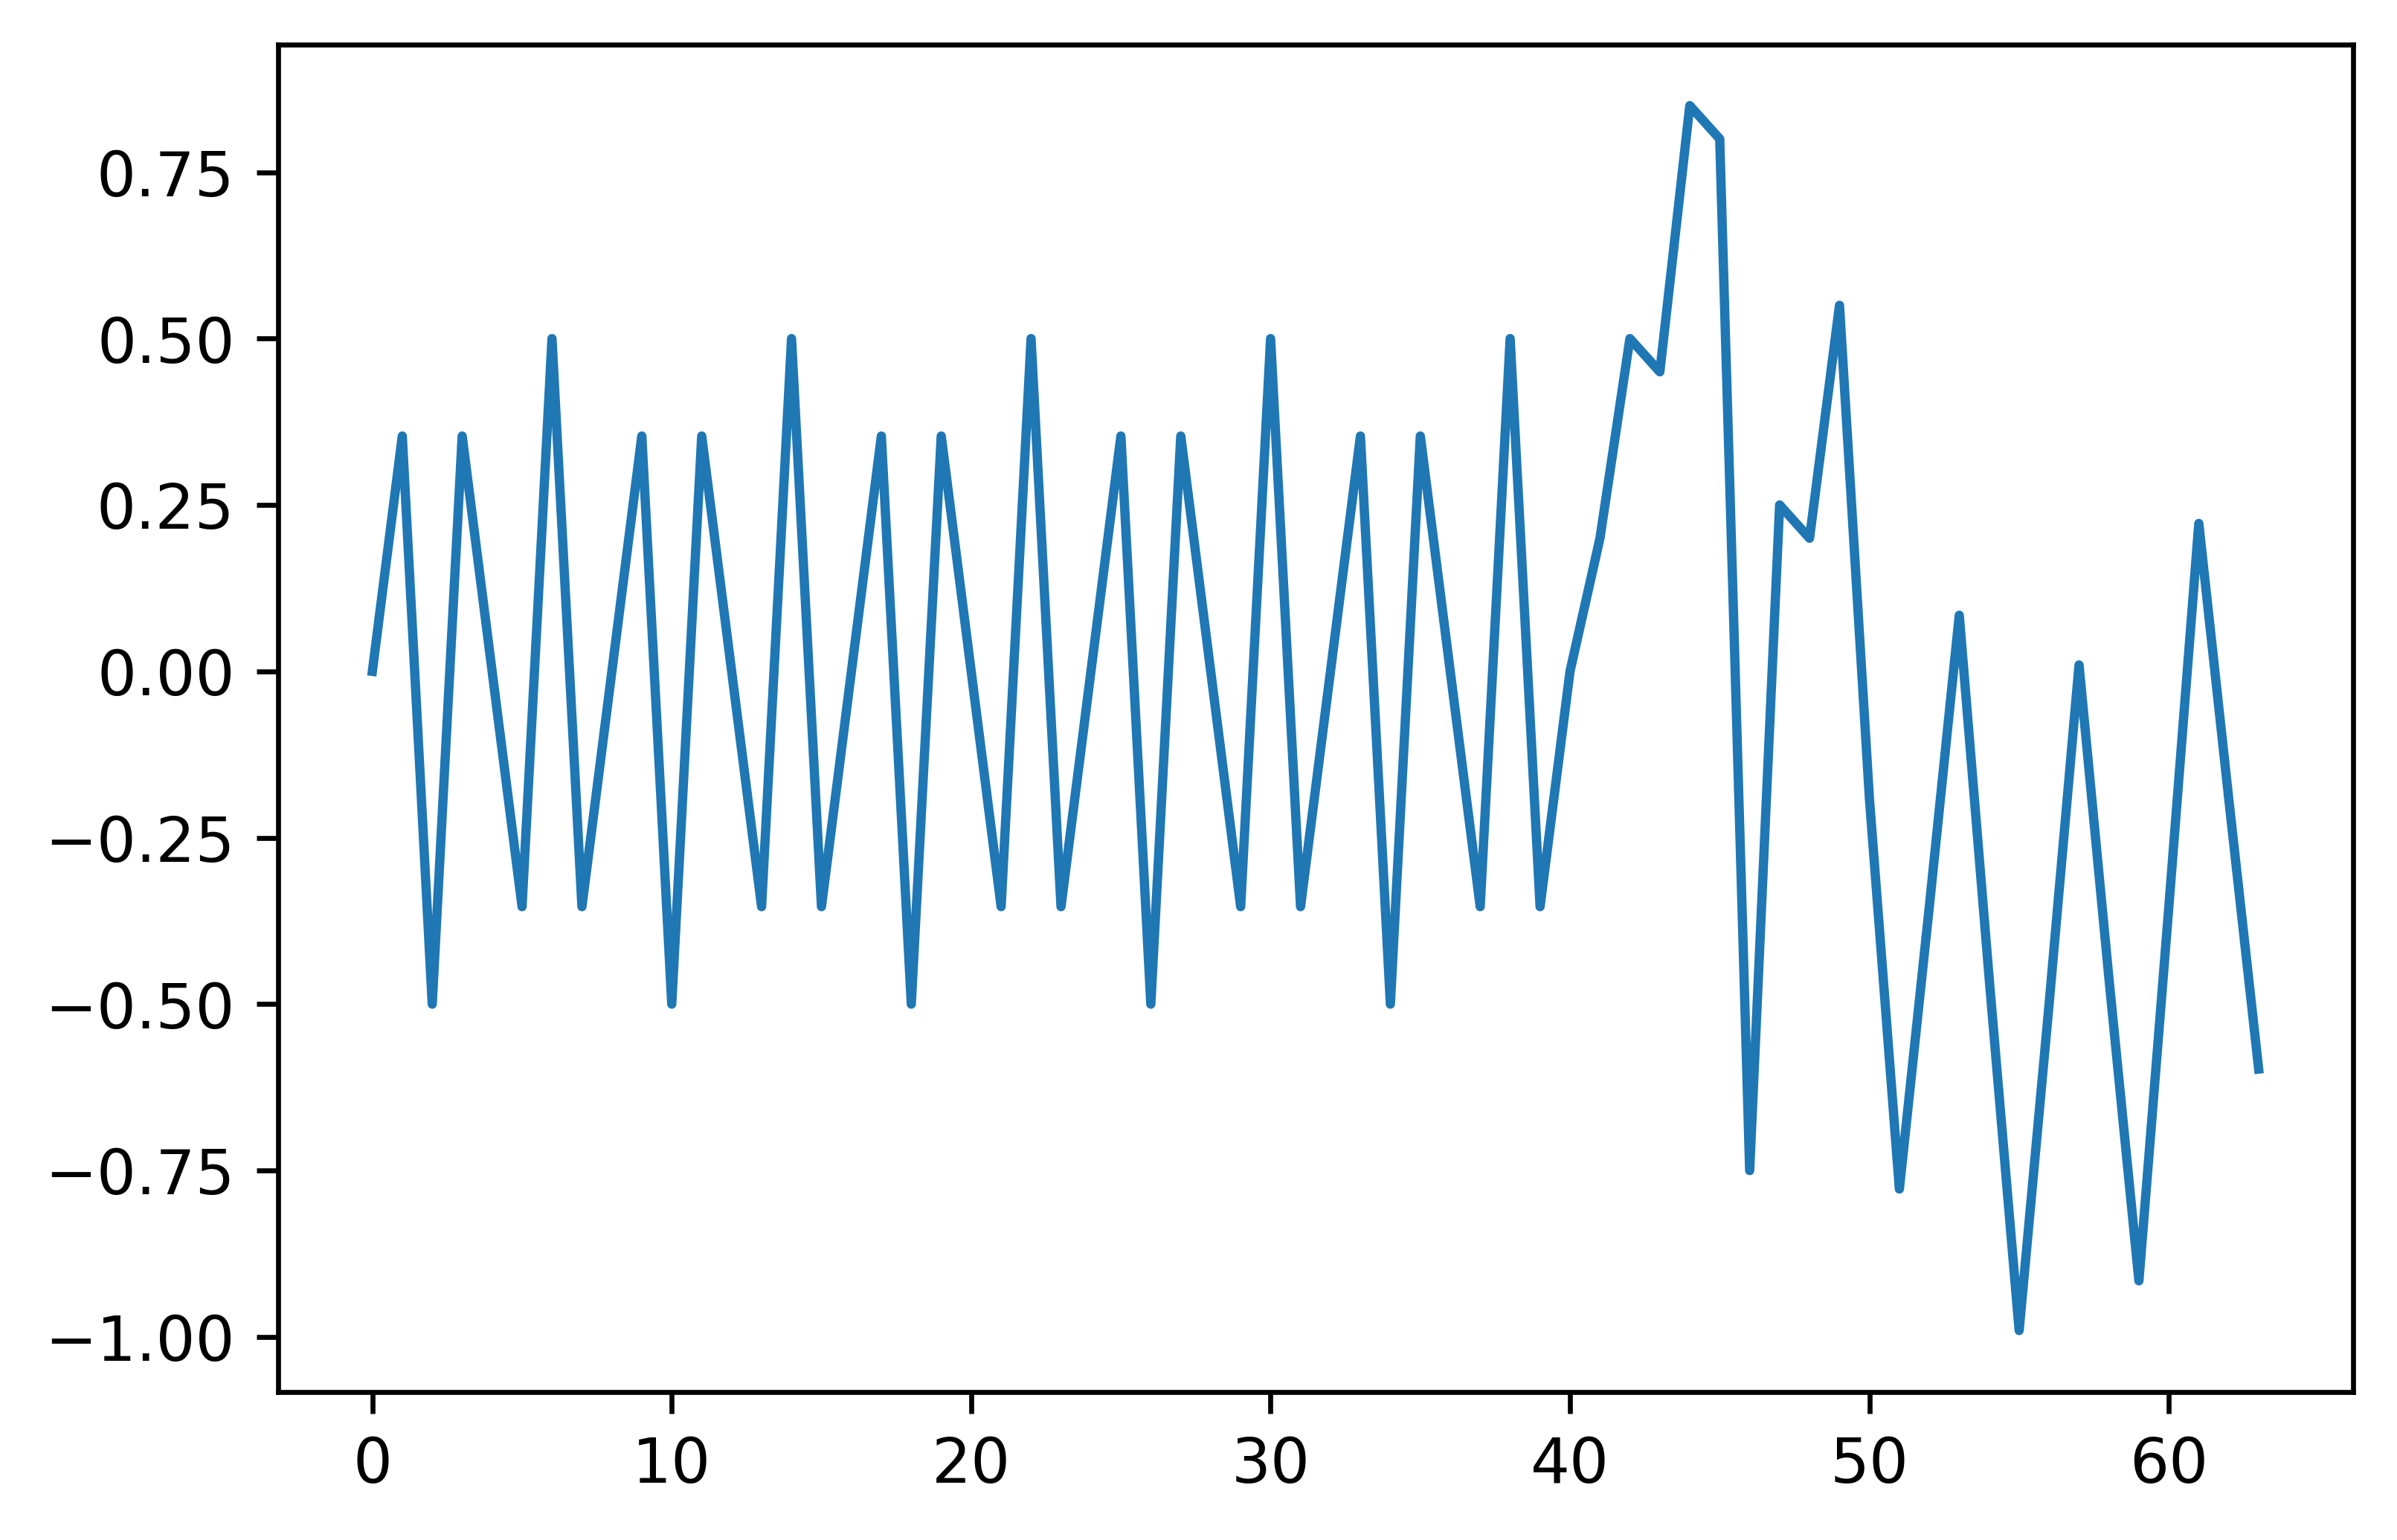
\includegraphics[scale=0.8]{Graphics/example-guido-signal.png}
	\caption{}
\end{figure}

La figura \ref{fig:example-guido-signal-dst-s} muestra el resultado de la DST-II sobre la señal $s[\cdot]$.
El gráfico color marrón es la sección \textit{second-rated} del resultado de ls DST-II sobre $s[\cdot]$.
El de color azul conrresponde a la heurística $S$ sobre los coeficiente de la \textit{second-rated}. 
La presencia de $m[\cdot]$ se confirma en la posición $22$ de la DST-II y de $S$, donde se alcanzan valores
cercanos a $0$ y a $1$ respectivamente. Este coeficiente corresponde aproximadamente a la posición 
$44$ en la señal original. Como se puede apreciar, existe un ligero desplazamiento en la posición donde se detecta $m[\cdot]$,
pero no es de gran tamaño.


\begin{figure}\label{fig:example-guido-signal-dst-s}
	\centering
	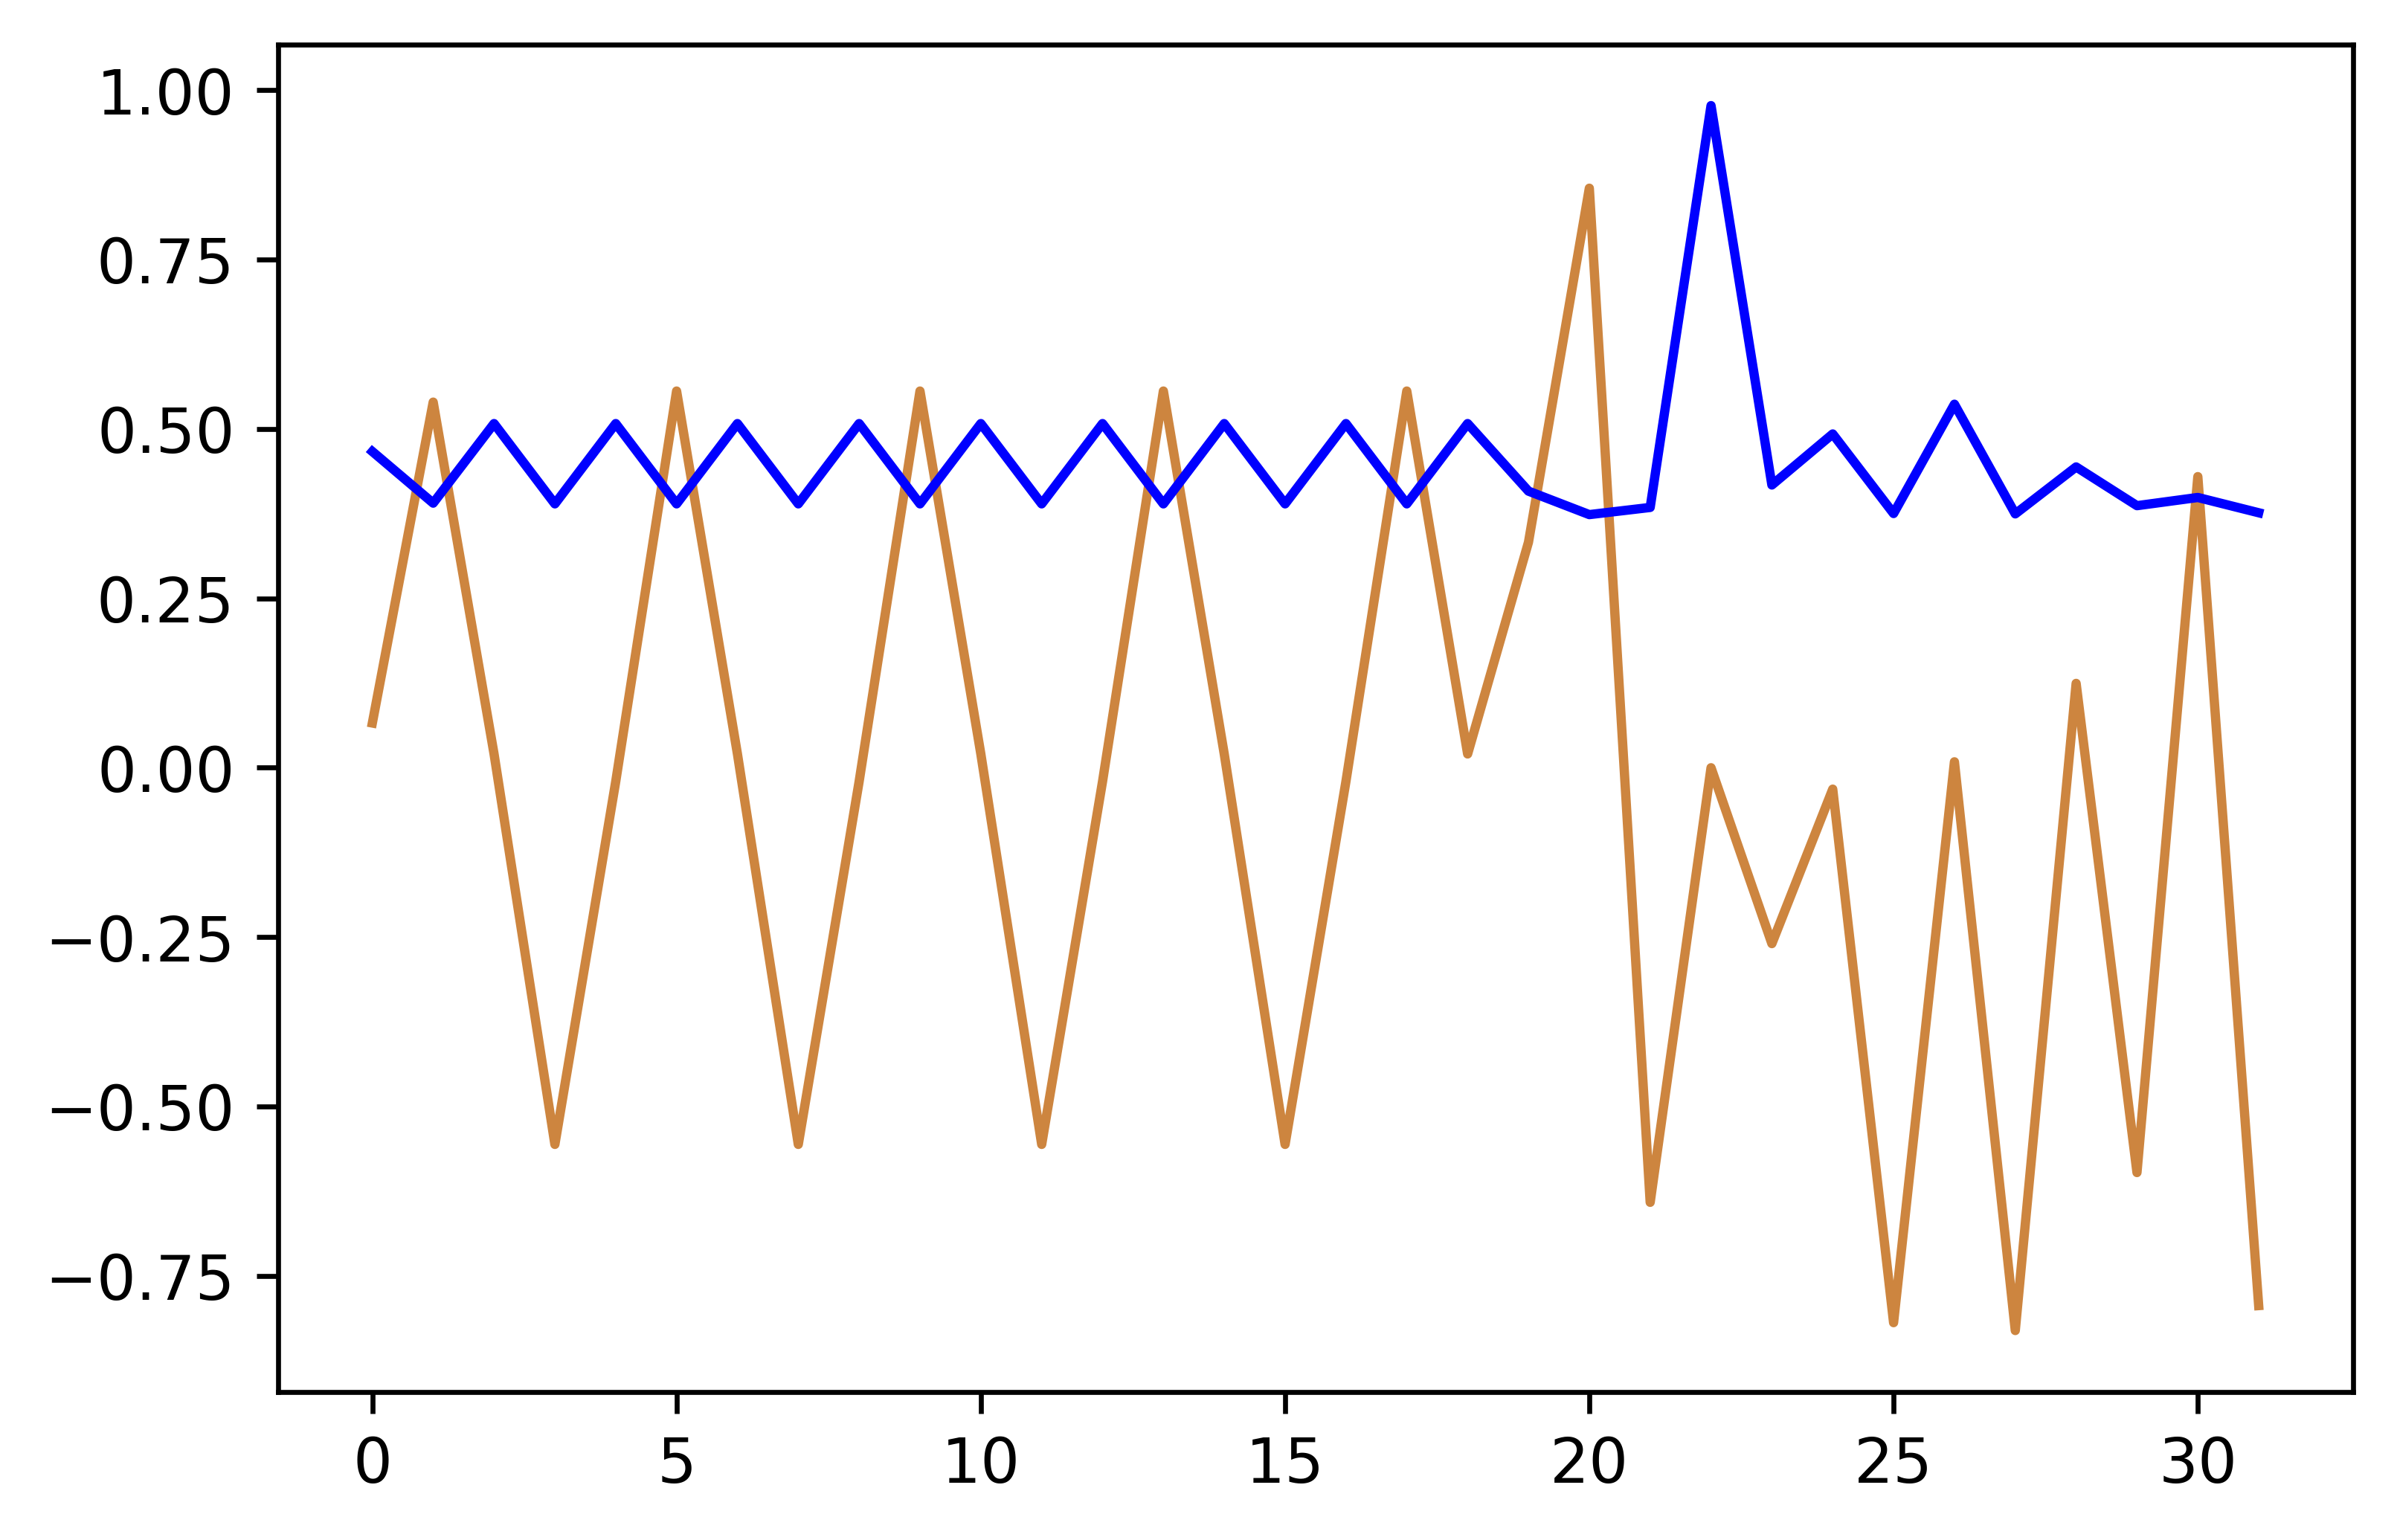
\includegraphics[scale=0.8]{Graphics/example-guido-signal-dst-s.png}
	\caption{}
\end{figure}


\section{Extensión de la DST-II para señales 2D}\label{section:2d}

La DST-II fue diseñada para el caso unidimensional. En este trabajo se busca experimentar sobre las formas en que
este algoritmo se puede extender al caso de de señales de bidimensionales. 
A continuación se exponen algunas ideas sobre la extensión de la DST-II para imágenes y la detección de patrones en este tipo de señales.

\subsection{Primer enfoque: DST-II por filas y luego columnas}

En \ref{section:dwt-2d} se explica como se extiende la DWT para el caso de dos dimensiones. Dado que la DST-II comparte 
muchas de las características de la DWT, se podría extender de esta misma forma para el caso bidimensional.
Cuando se busca extender la DST-II para el caso de imágenes lo que se quiere aprovechar es su capacidad
de detectar formas y patrones. 

La heurística \ref{eq:s-heuristic} se puede, en principio, extender para el caso de señales bidimensionales también.
Solo que este caso una mejor forma de visualizar la detección sería con un mapa de colores para cada uno de los coeficientes
de la transformada.

Dado que se está trabajando con imágenes y secciones de las mismas se va a usar de ahora en adelante la notación
$[A:B,C:D]$ para describir una región o porción de la imagen. $A$ y $B$ representan el intervalo en las filas
comprendidos entre dichos valores. De forma similar lo hacen $C$ y $D$, pero para las columnas.



\begin{figure}\label{fig:gaussian-example-dst}
	\centering
	\subfigure[Imagen]{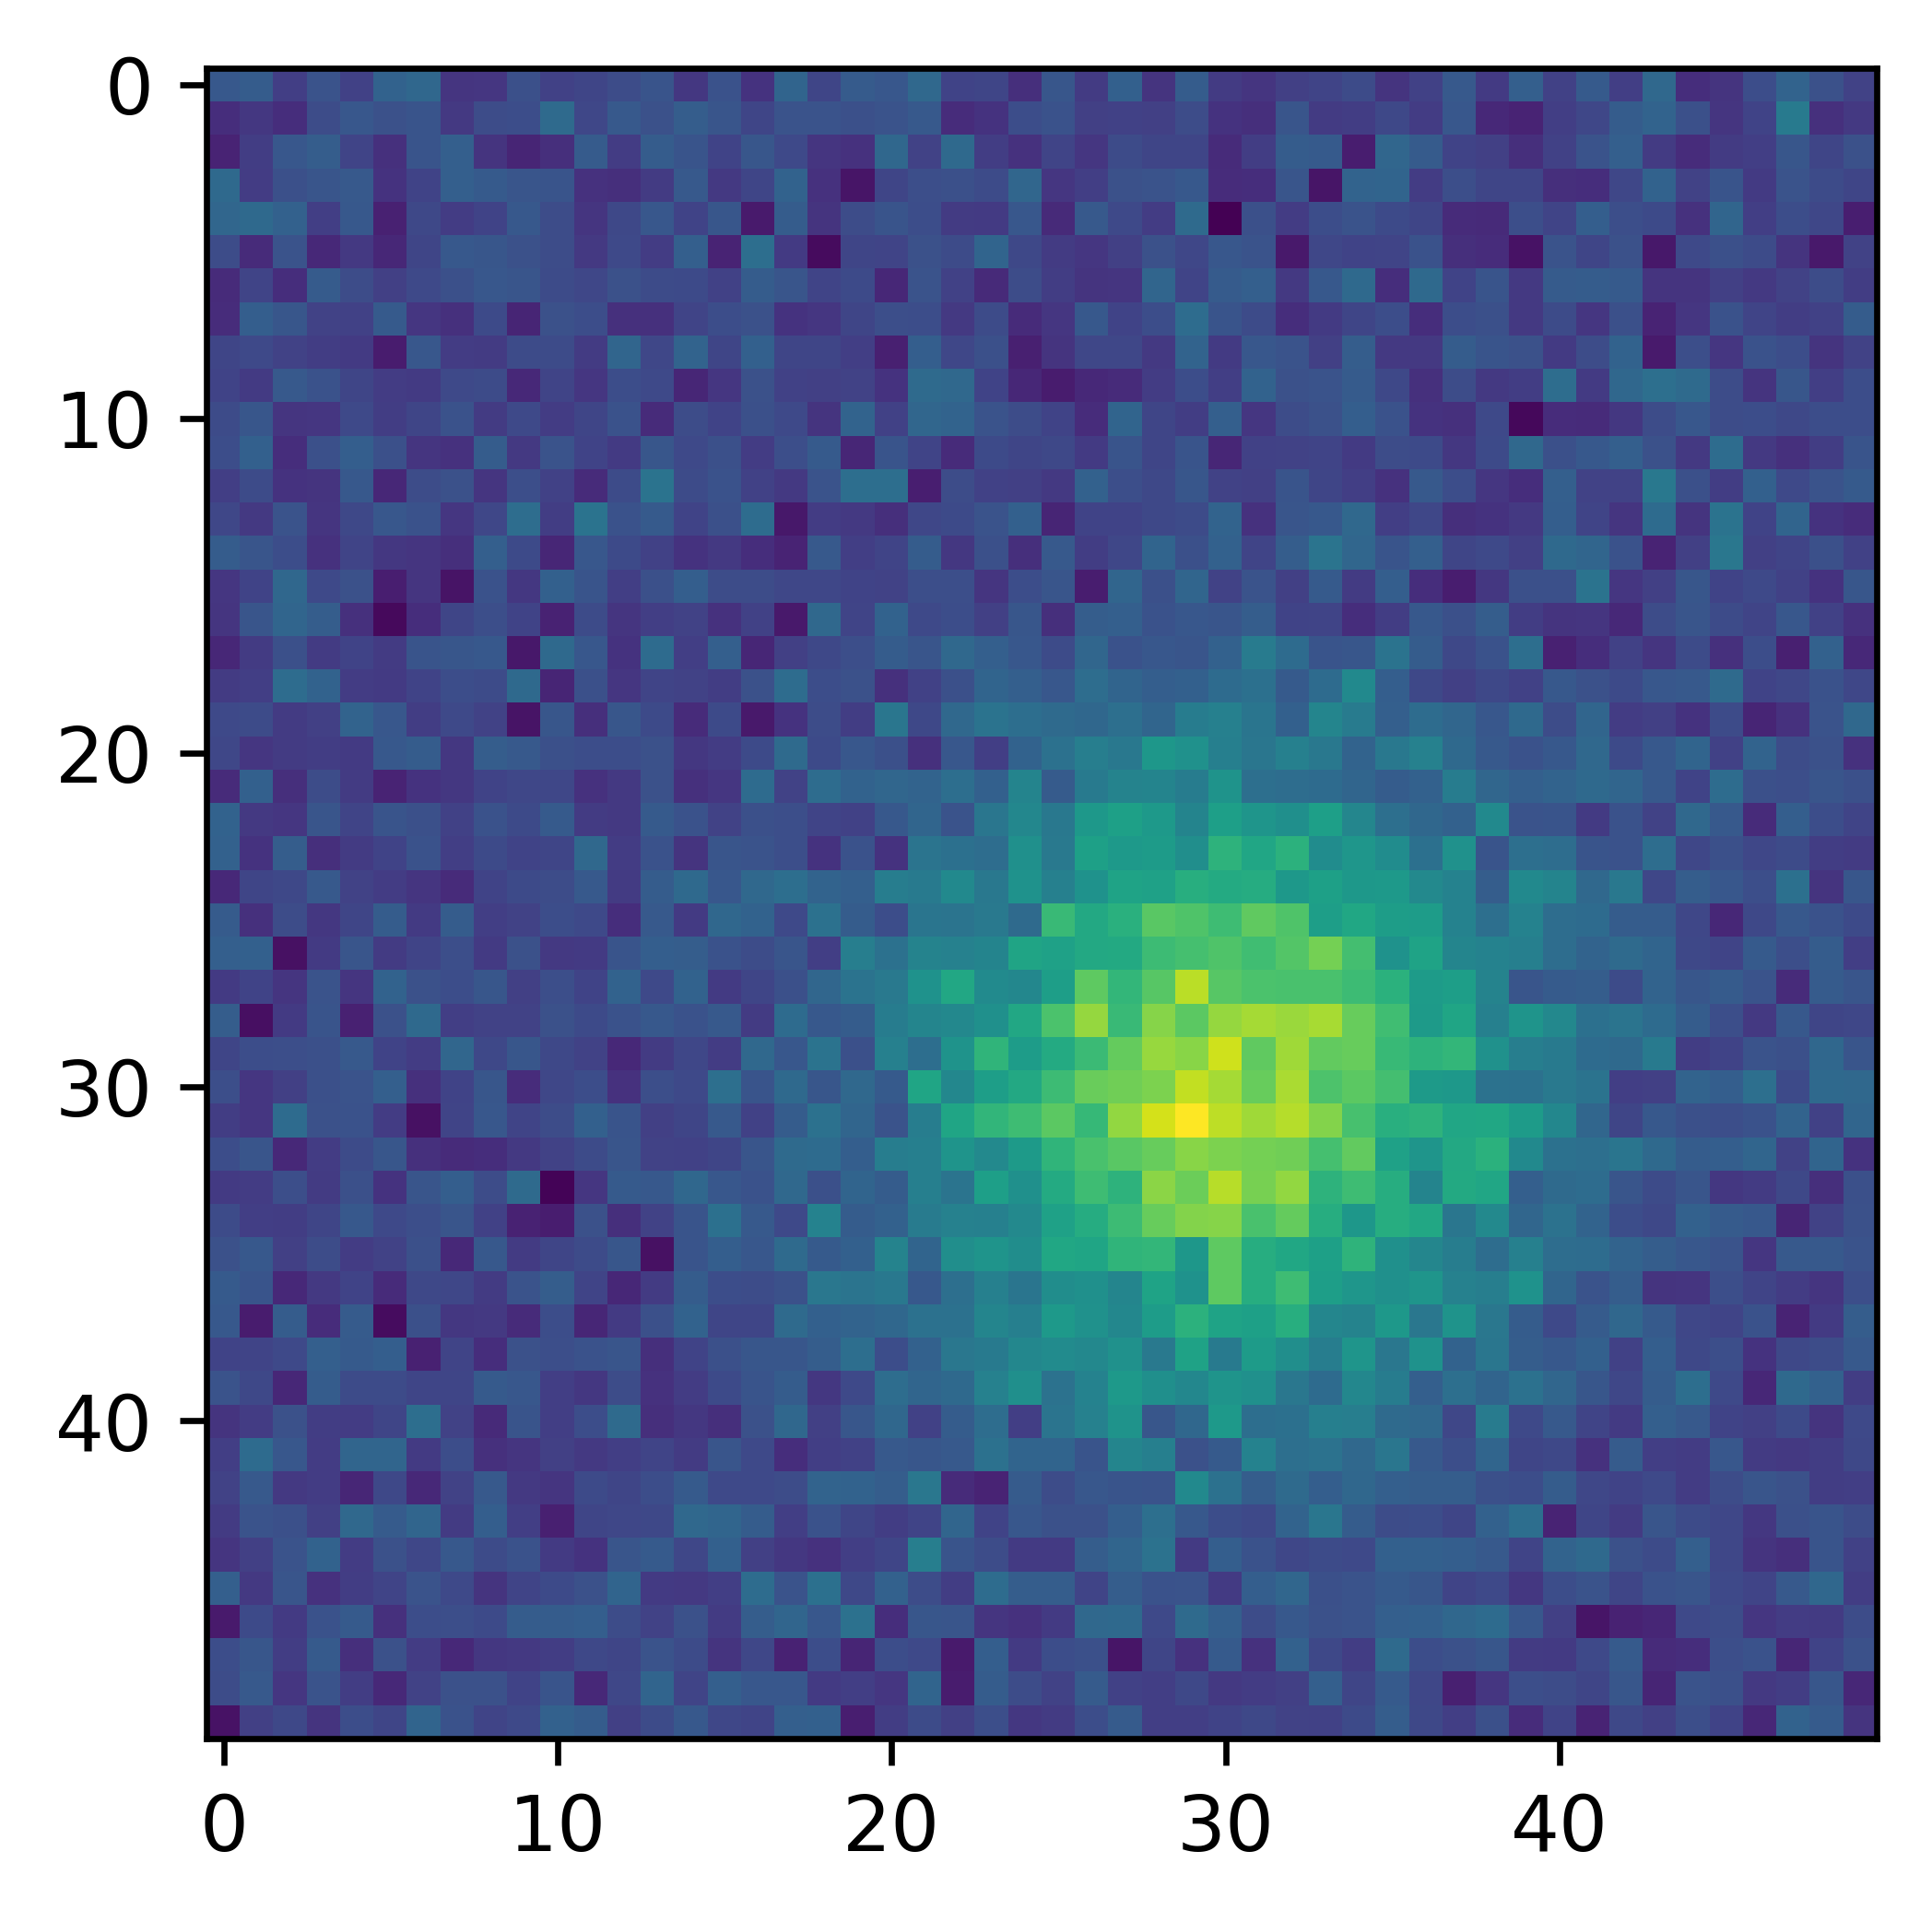
\includegraphics{Graphics/gaussian-example-dst.png}}
	\subfigure[Patrón]{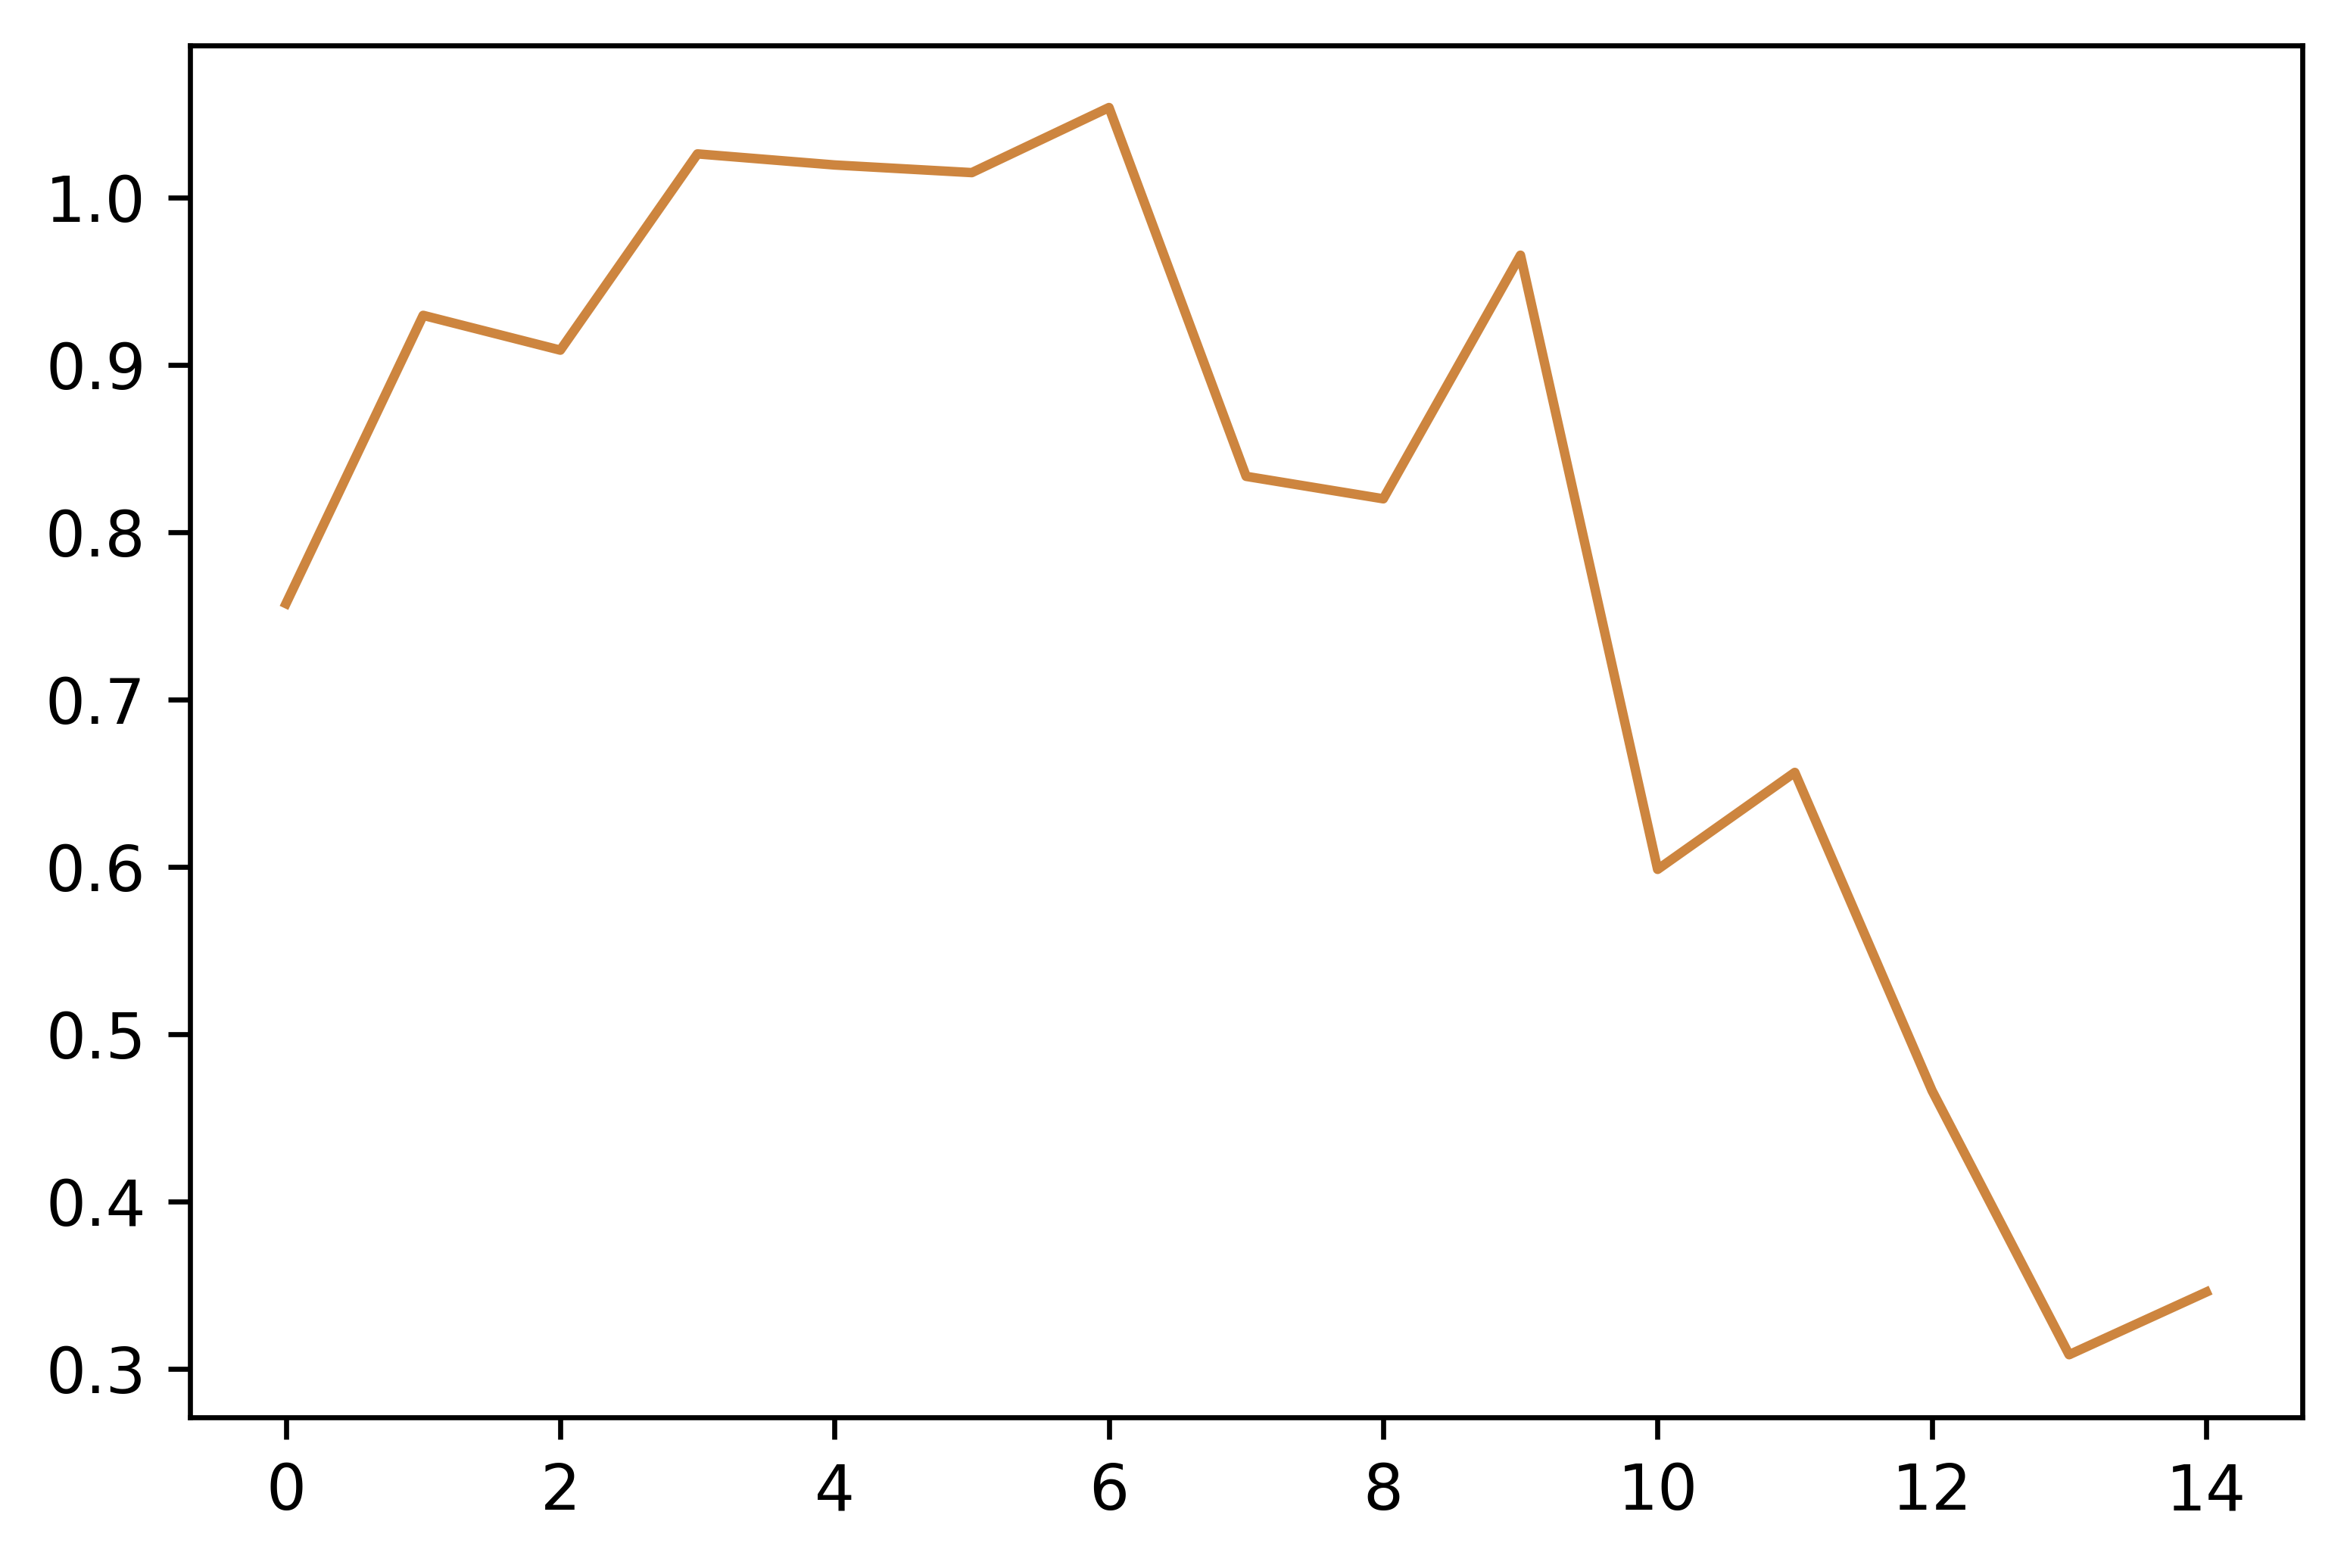
\includegraphics{Graphics/example-line-pattern-dst.png}}
	\caption{Imagen de una gaussiana y sección correspiende a los pixeles [30, 25:40] }
\end{figure}

\begin{figure*}\label{fig:dst-gaussian-example}
\begin{multicols}{2}
    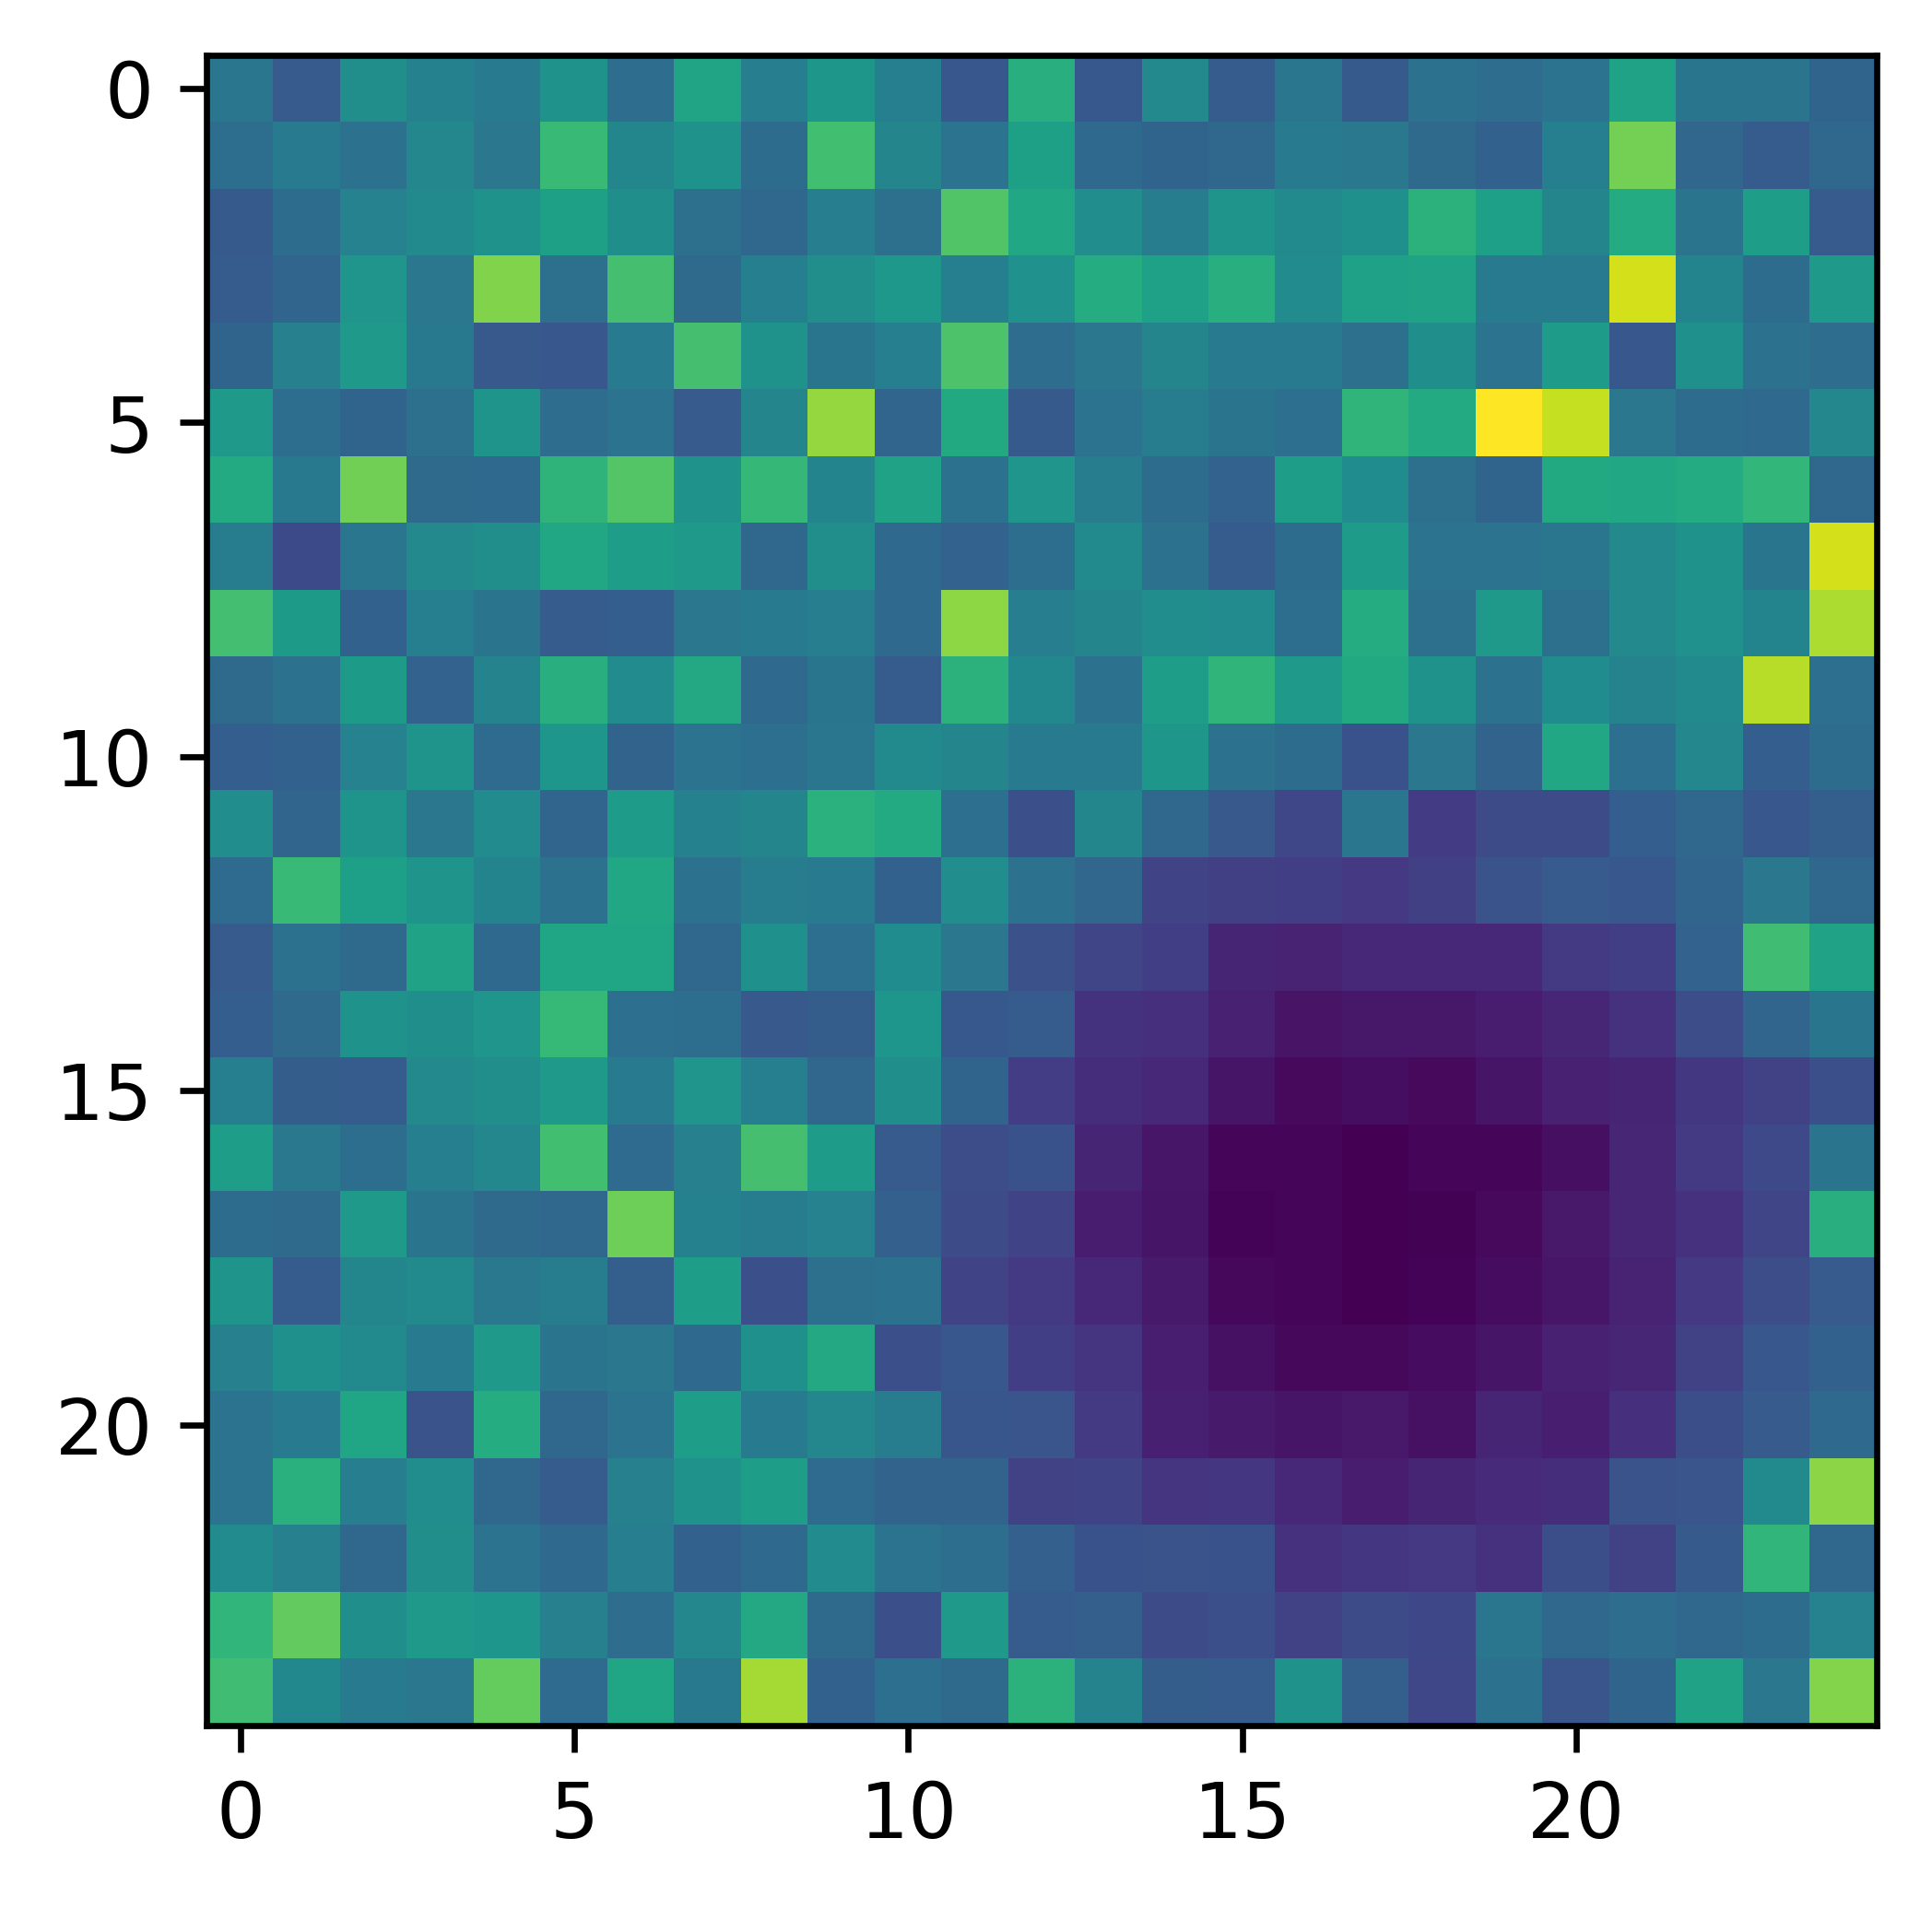
\includegraphics[width=\linewidth]{Graphics/gaussian-example-aproximation-dst.png}\par 
    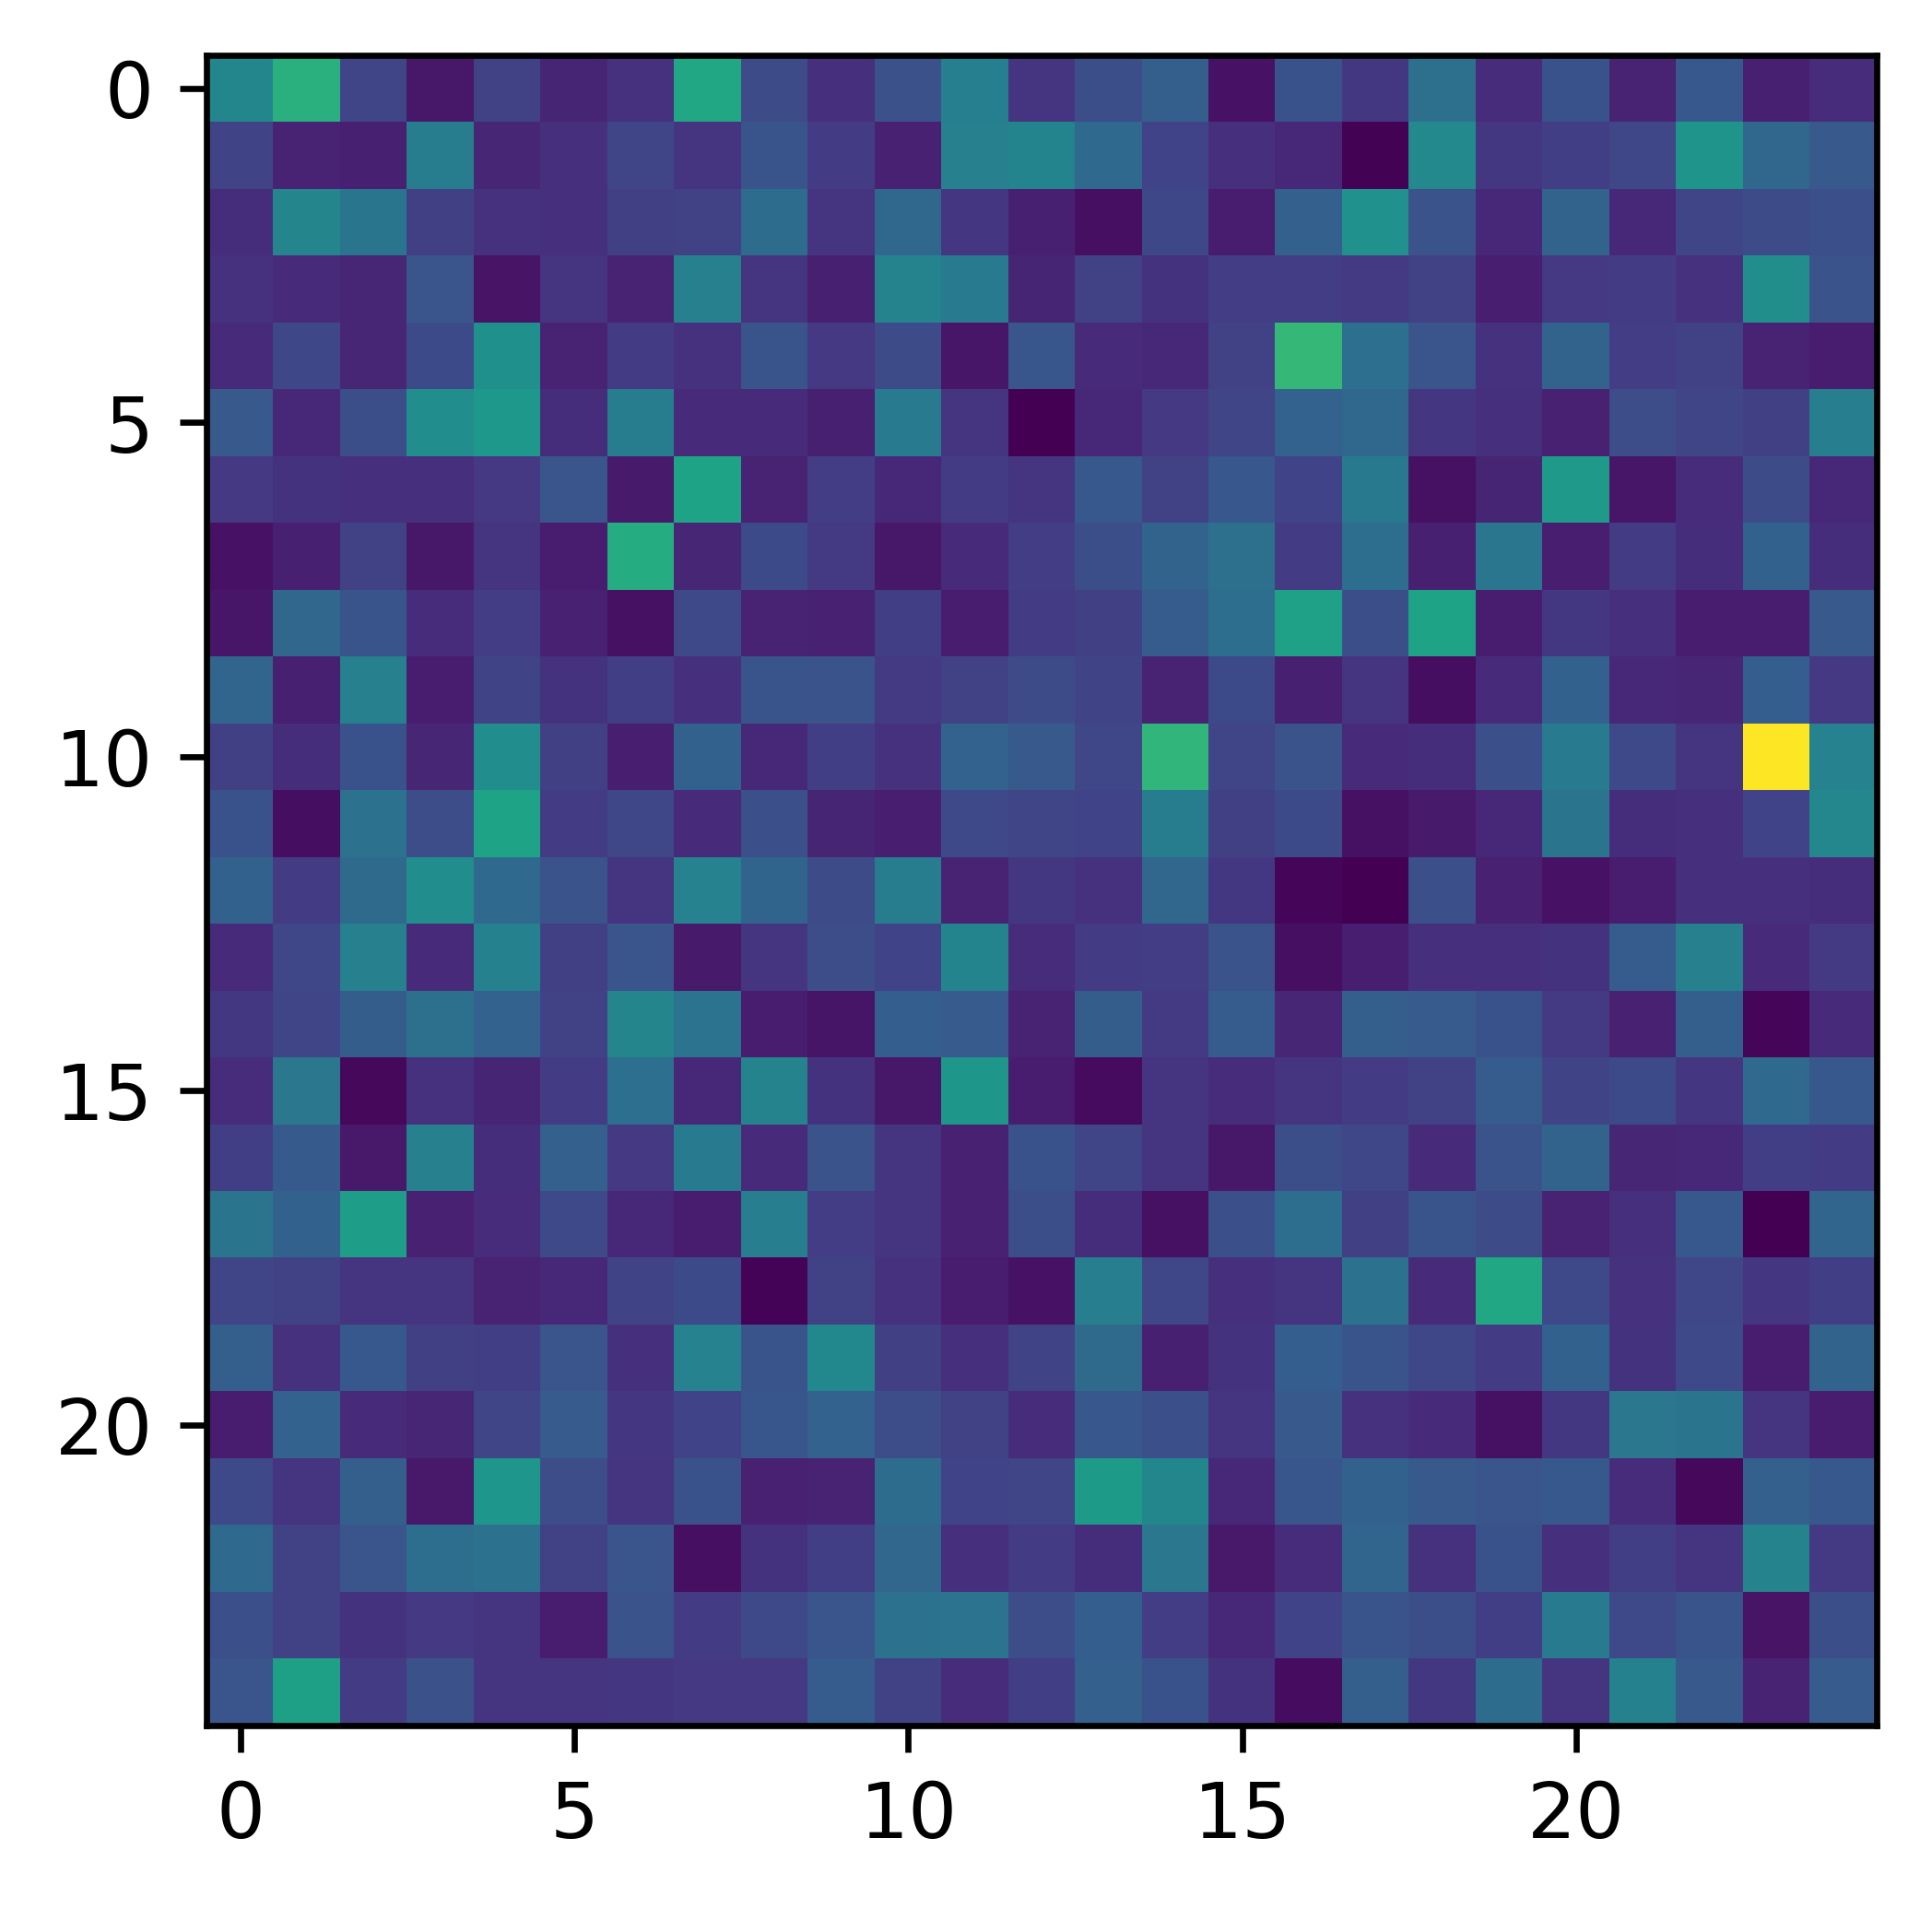
\includegraphics[width=\linewidth]{Graphics/gaussian-example-horizontal-dst.png}\par 
    \end{multicols}
\begin{multicols}{2}
    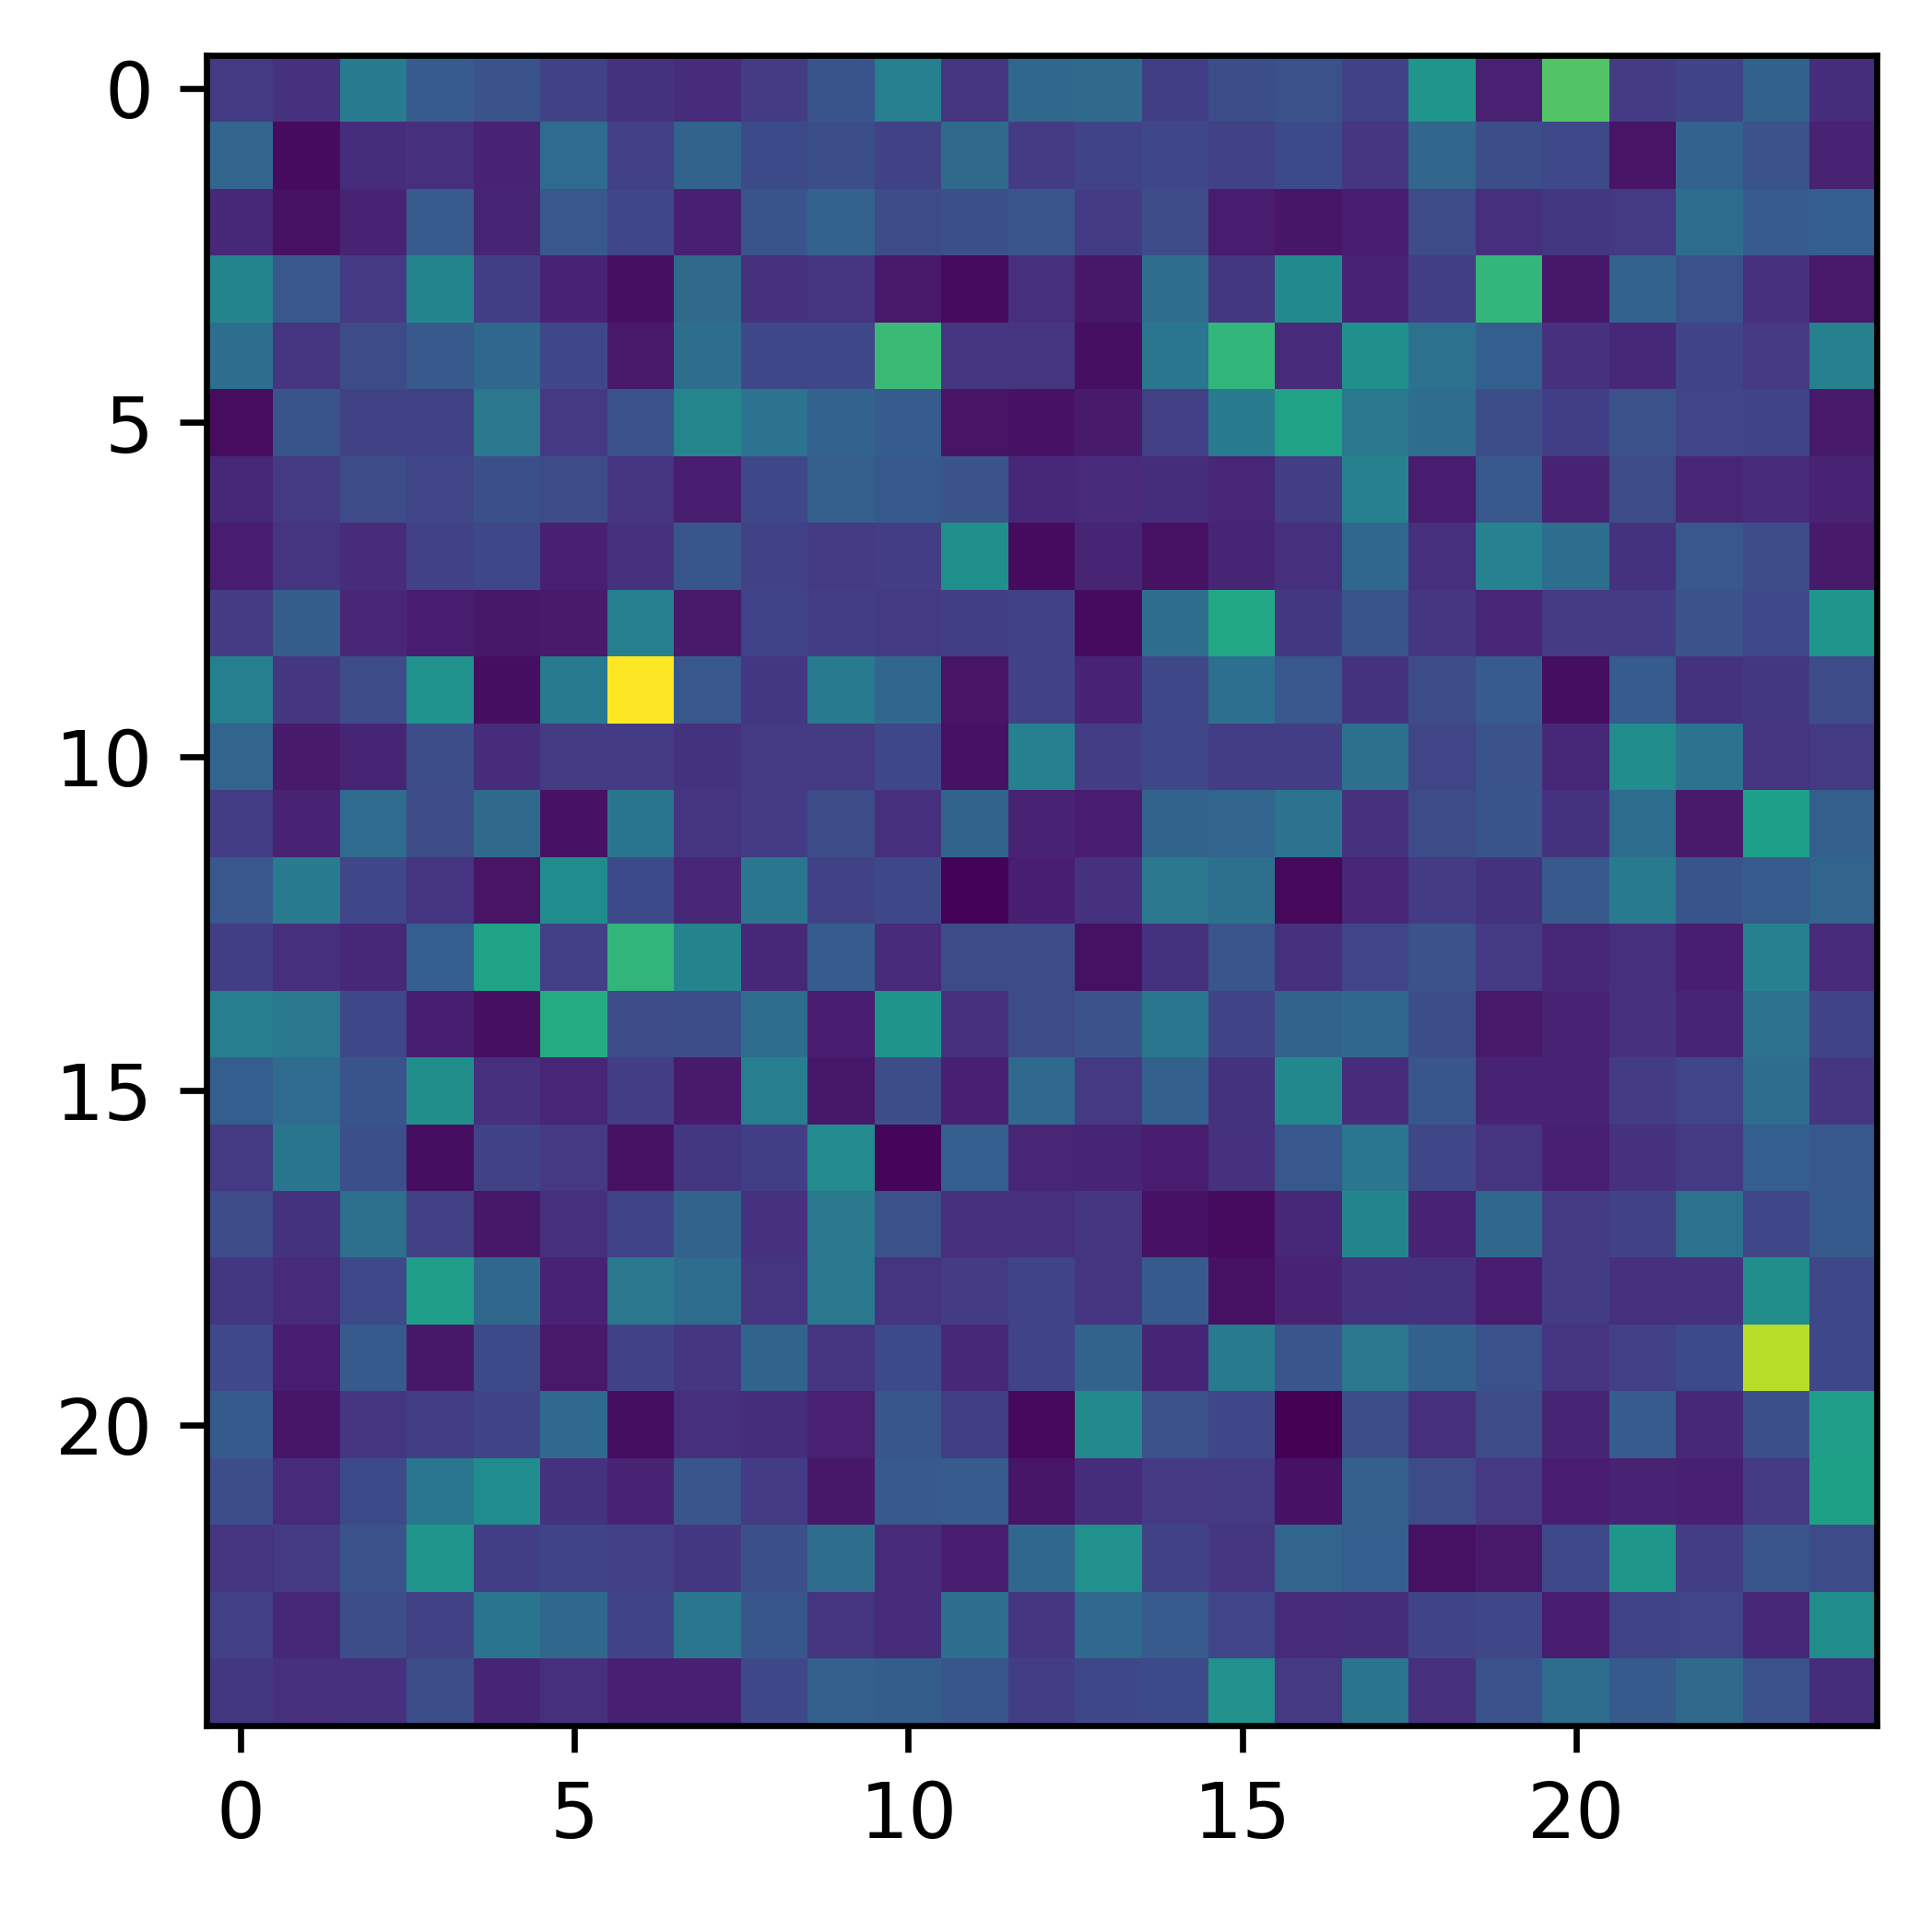
\includegraphics[width=\linewidth]{Graphics/gaussian-example-vertical-dst.png}\par
    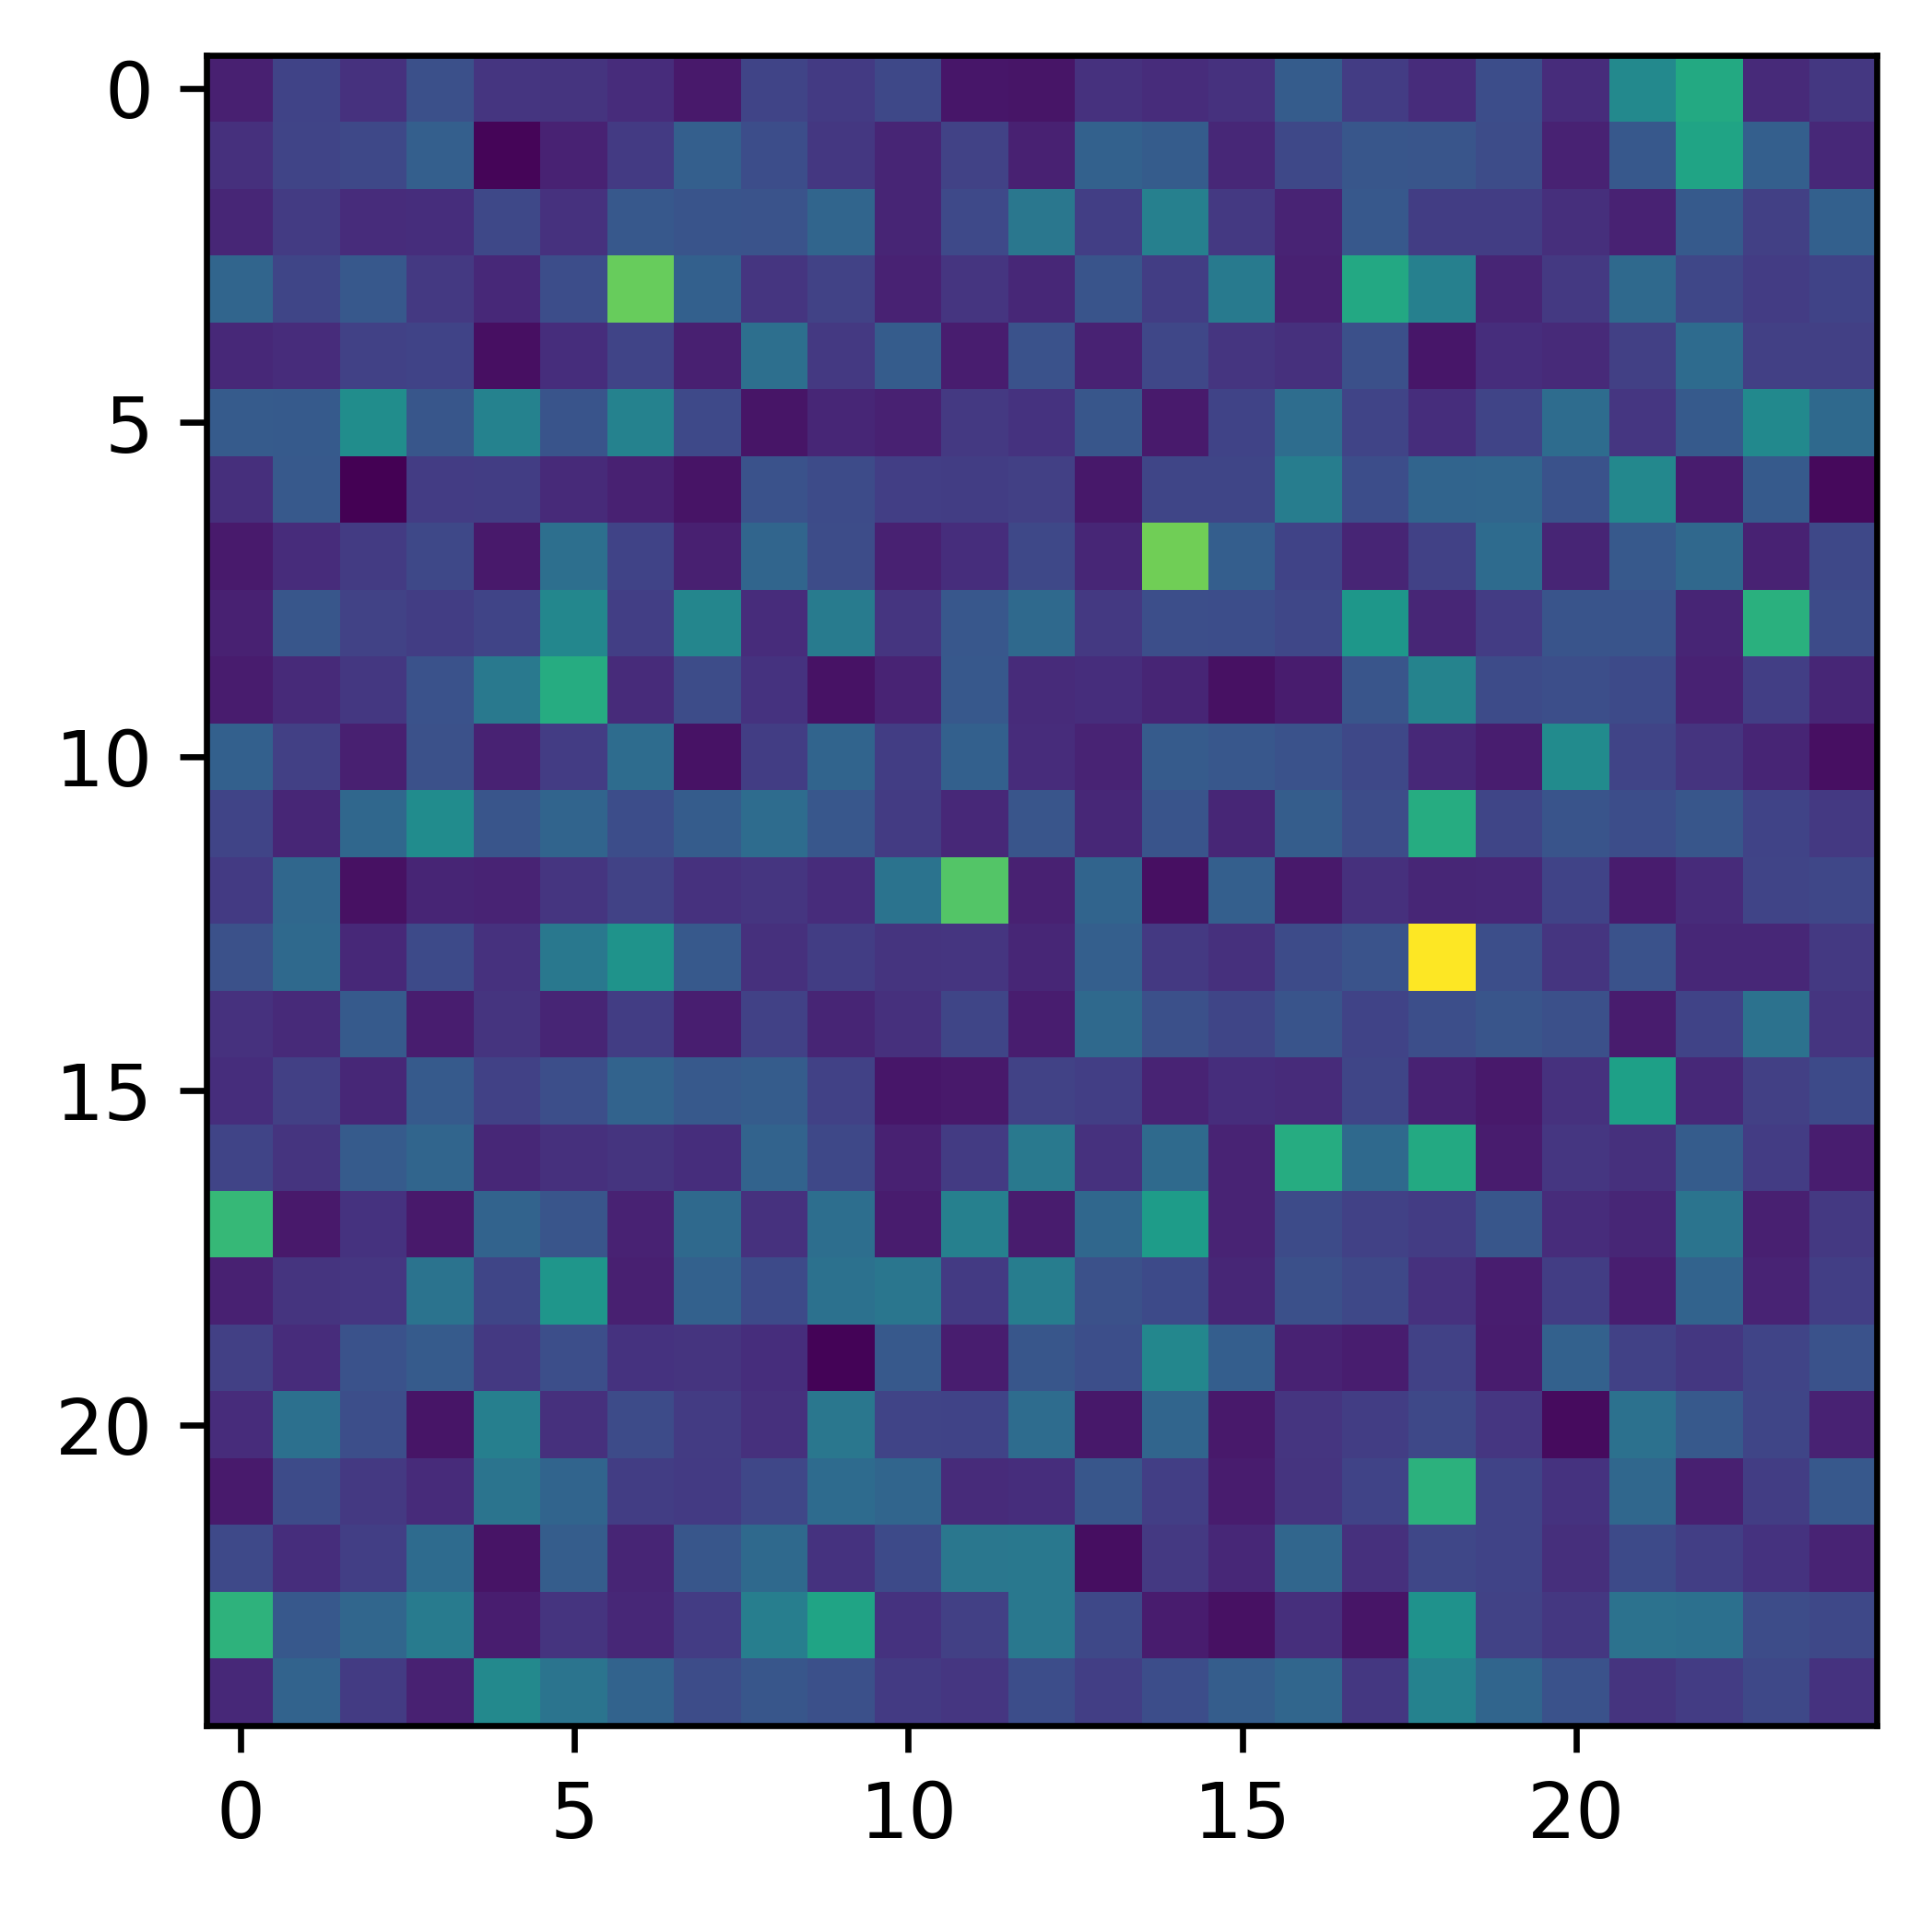
\includegraphics[width=\linewidth]{Graphics/guassian-example-diagonal-dst.png}\par
\end{multicols}
\caption{ Resultado de evaluar la función $S$ sobre cada de uno de los coeficiente de la DST-II contruida a partir del 
patrón \ref{fig:gaussian-example-dst} y sobre la misma imagen de donde se extrae el patrón}
\end{figure*}

La figura \ref{fig:dst-gaussian-example} muestra el resultado de hacer la DST-II siguiendo el procedimiento \ref{algoritmo:dst-2}.
El patrón tomado para la constucción de la DST-II es mostrado en la figura \ref{fig:dst-gaussian-example} que corresponde
a la sección $[30, 25:40]$ de la imagen. La transformada se realiza luego sobre esta propia imagen. El resultado que
es luego evaluado en la función $S$, para la detección de la posición del patrón.

Los coeficientes de aproximación no son de interés para la detección. Nótese que la DST-II realizaba la detección en la sección
\textit{second-rated}, que este caso correspondería a los coeficientes de detalle. En los coeficientes de detalle horizontal 
y vertical se ven puntos que sobresalen. Sin embargo, ninguno corresponde a posiciones donde está localizado el patrón 
a partir del cual se construyó la shapelet. En el caso de los coeficiente de detalle diagonal, se detecta un punto por la
herística $S$ en la posición $(13,18)$ con valor $0.7239220309171849$. Este coeficiente corresponde a la posición
$(26,36)$ de la imagen original. La ubicación real del patrón es la fila $30$, entre las columnas $25$ y $40$. Por lo que
parece ser al menos el resultado de la heurística sobre los coeficientes de detalles diagonal da como resultado una 
aproximación de donde termina el patrón. 


\subsection{Segundo enfoque: DST-II solamente por filas (columnas)}

Otra forma de extender la DST-II al caso de señales bastante sencilla  es realizar la transformada 
una sola vez, es decir, por filas o por columnas solamente.

El primer paso sería seleccionar la señal o patrón que se quiere detectar, y la dirección.
Tomando la misma la sección horizontal del patrón $[30, 25:40]$ y realizando la DST-II solamente por filas 
se obtiene el punto en la posición $(30, 16)$ con valor de $S=0.9830214409852203$. Esta posición corresponde 
a la fila $30$ y a aproximadamente a la columna $32$ de la imagen original. La figura
\ref{fig:gaussian-example-dst-rows} muestra el resultado.

\begin{figure}\label{fig:gaussian-example-dst-rows}
	\centering
	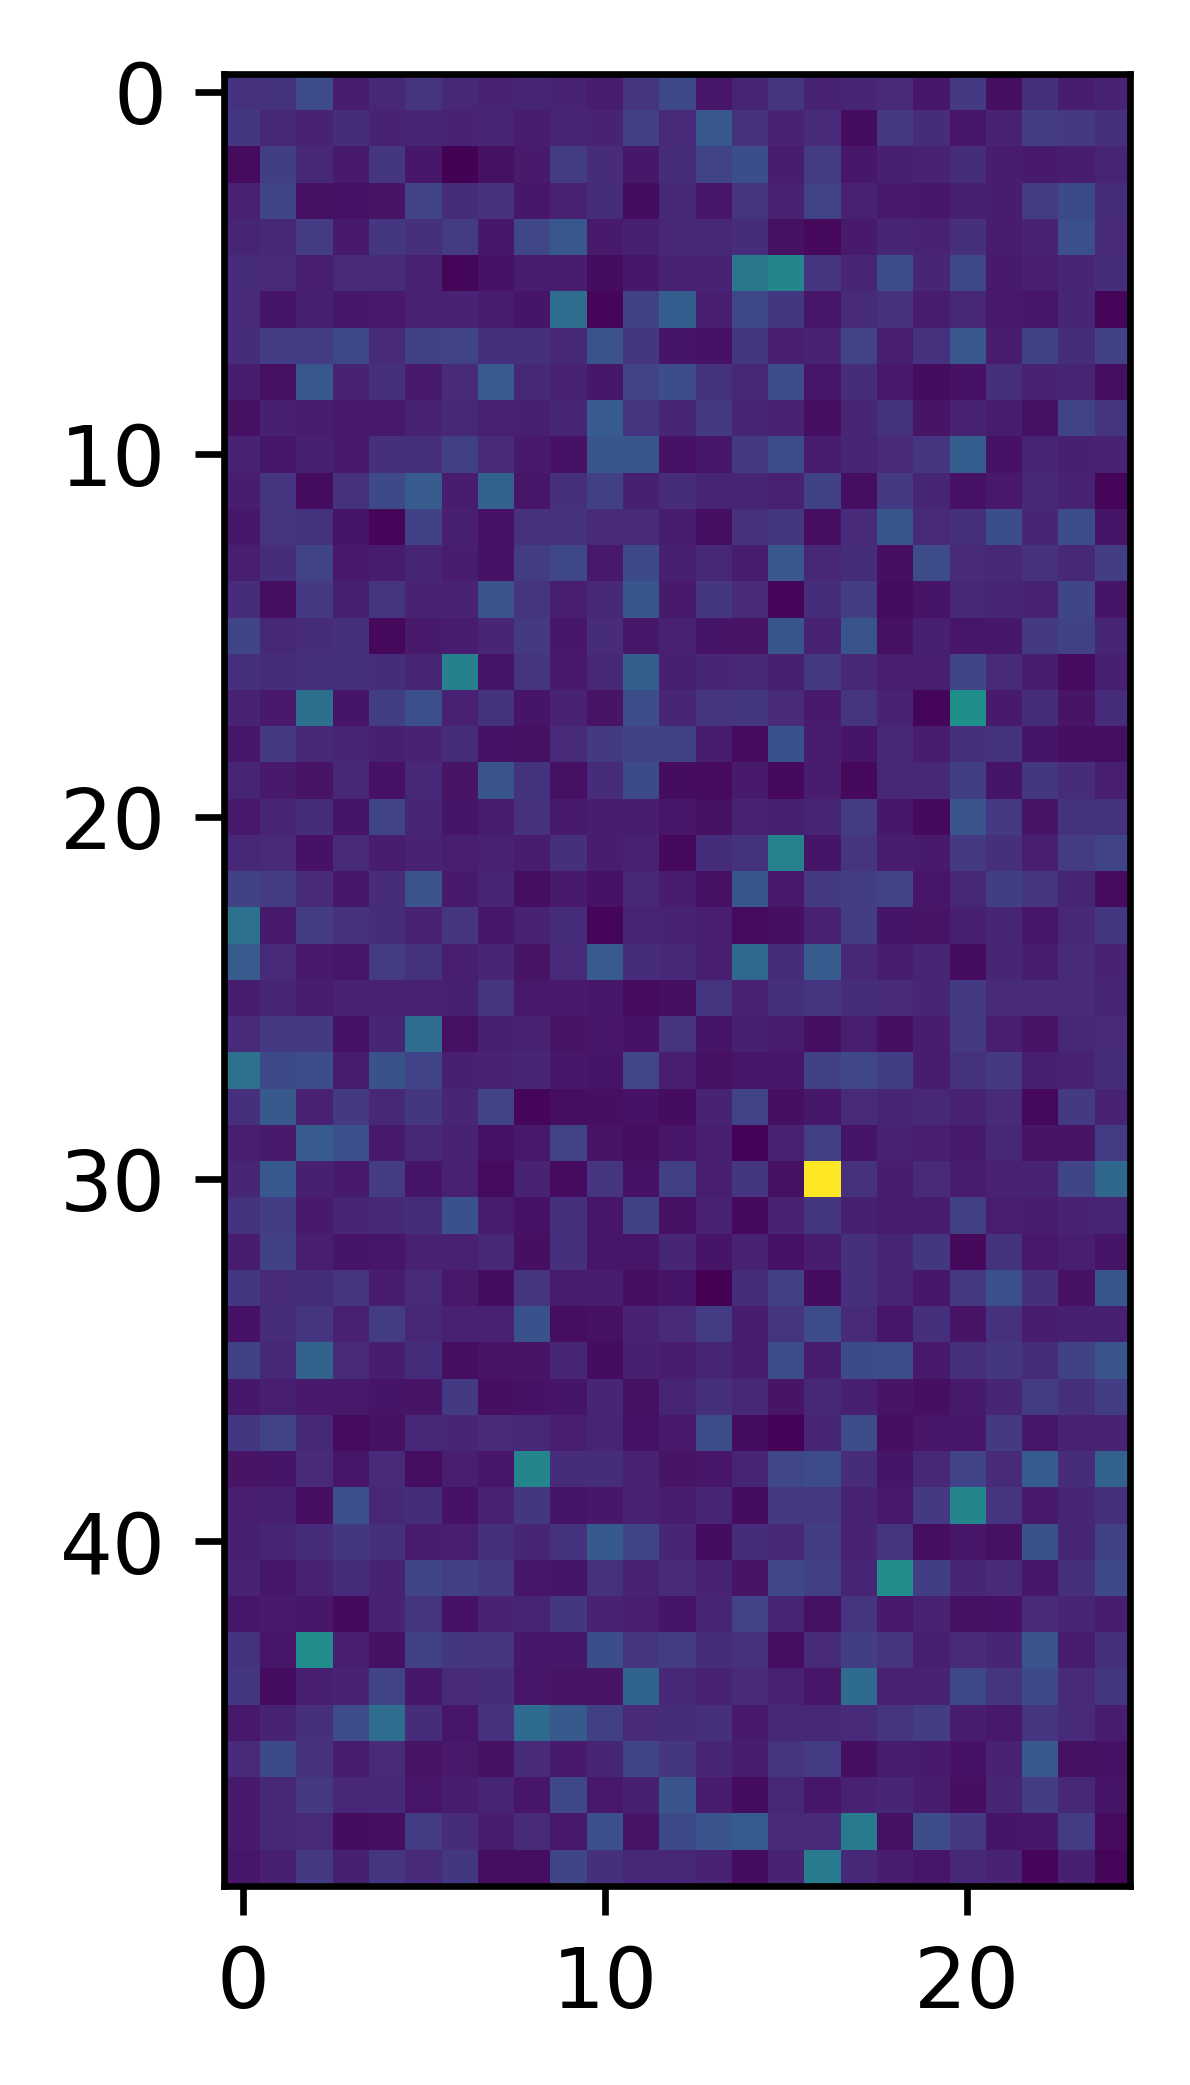
\includegraphics{Graphics/gaussian-example-dst-rows.png}
	\caption{Imagen de una gaussiana  }
\end{figure}

Como se puede apreciar, en las filas el resultado es exacto, pero en las columnas existe un pequeño error con respecto
a la posición donde empieza el patrón. Para poder contrarrestar esto se puede tomar una sección vertical del patrón
y proceder de forma análoga a como se hizo con las filas. En este caso se toma la sección vertical del patrón
correspondiente a las posiciones $[24:37, 30]$. La figura \ref{fig:gaussian-example-dst-cols} muesta el resultado

\begin{figure}\label{fig:gaussian-example-dst-cols}
	\centering
	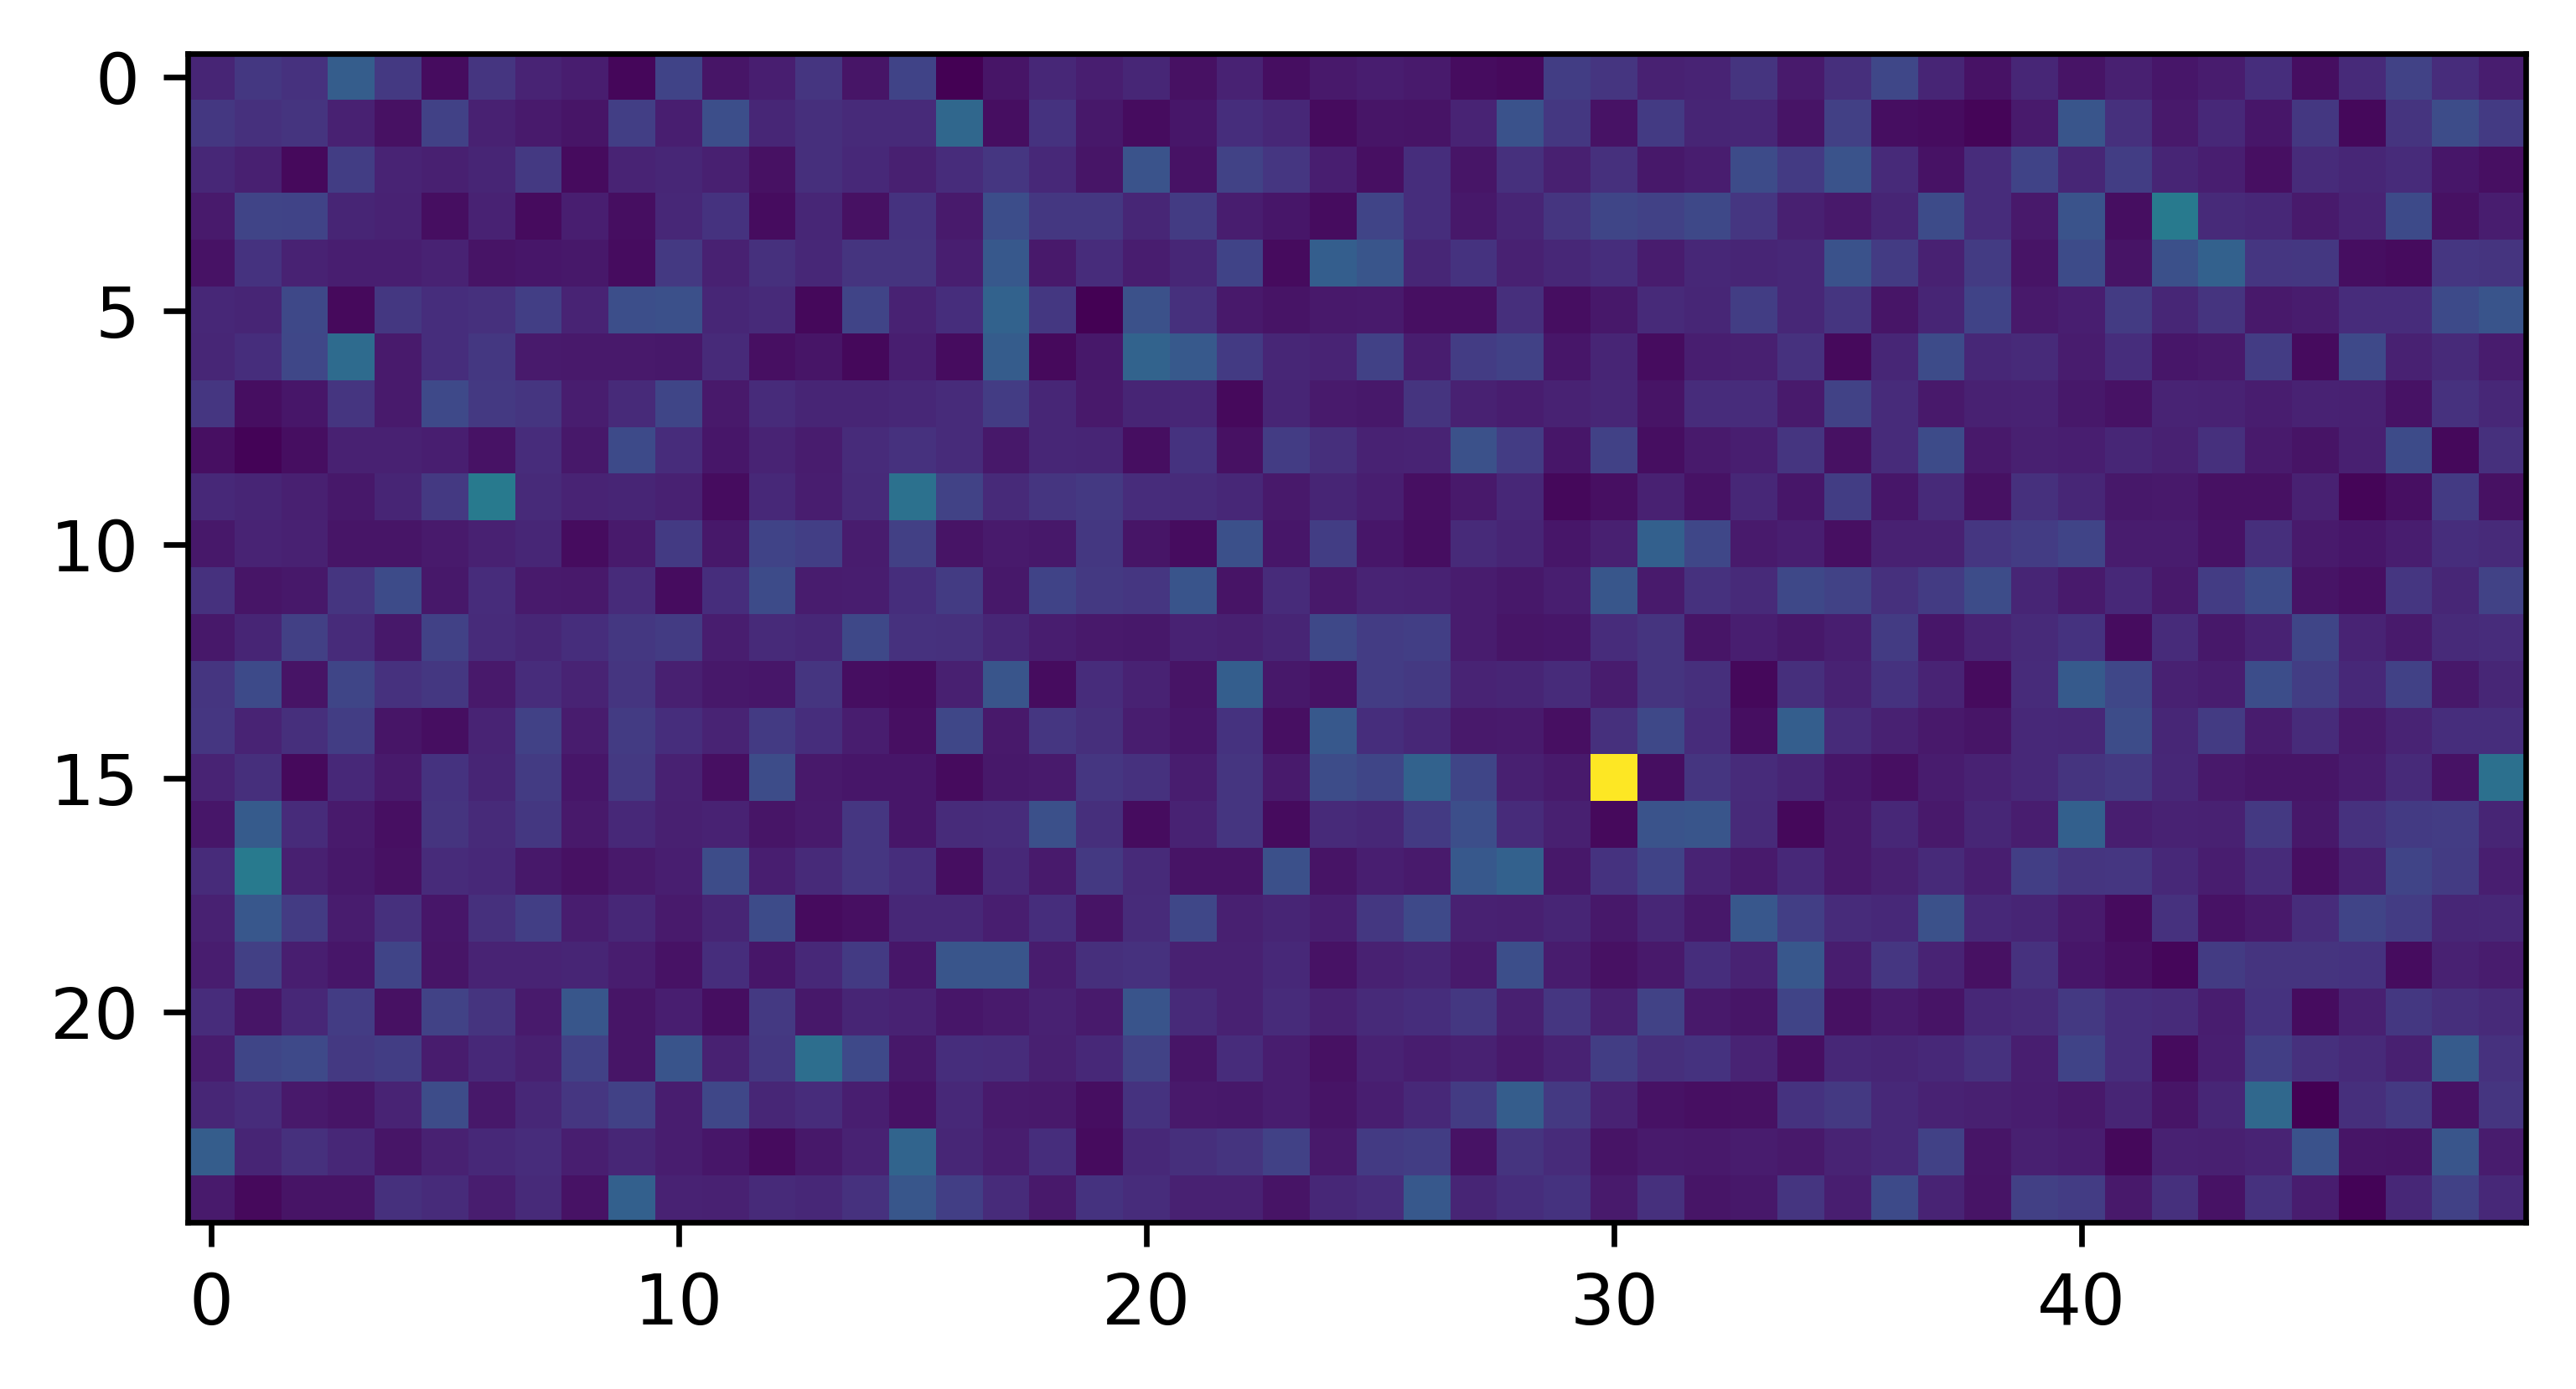
\includegraphics{Graphics/gaussian-example-dst-cols.png}
	\caption{Imagen de una gaussiana  }
\end{figure}

La detección se realizó en el punto $15, 30$ con un valor de $S=0.9763538820250564$, que corresponde a la fila 
$30$ aproximadamente y a la columna $30$.

Juntando la información de ambas transformadas es posible lograr una detección más exacta de donde empieza el patrón 
que se quiere encontrar. Por este motivo, se recomienda entonces tomar un line profile vertical y otro horizontal
para obtener más información durante el proceso de detección.

\subsection{Tercer enfoque: DST-II usando varias shapelets}

Como se muestra en la sección anterior, mientras más secciones del patrón se tomen, más información sobre la detección se puede
obtener. Dado que en muchas apliaciones los patrones que se quieren encontrar pueden estar contenidos en imágenes
con mayores dimensiones, obtener la posición a nivel de un solo par de píxeles no es cómodo. De hecho, lo que se buscaba en
principio con esta investigación era ver si podía lograr un mejoramiento del constraste en la región donde se detecta el
patrón. Por este motivo, se propone otra alternativa al enfoque anterior que consisite en usar varias shapelets 
para la detección y promediar los resultados de todas. Con esta técnica lo que se buscar es lograr detectar
el contorno donde se detectan las distintas partes del patrón.
